%%%%%%%%%%%%%%%%%%%%%%%%%%%%%%%%%%%%%%%%%%%%%%%%%%%%%%%%%%%%%%%%%%%%%%%%%%%
\section{Production Plan}
\label{sec:fdsp-apa-prod}
%%%%%%%%%%%%%%%%%%%%%%%%%%%%%%%%%%%%%%%%%%%%%%%%%%%%%%%%%%%%%%%%%%%%%%%%%%%

The \dword{apa} Consortium oversees the design, construction, and testing of the \dword{dune} \dword{spmod} \dwords{apa}. Production sites are being planned in the USA and UK. This approach allows the consortium to produce \dwords{apa} at the rate required to meet overall construction milestones and, at the same time, reduce risk to the project if any location has problems that slow the production pace.

The starting point for the \dword{apa} production plan for \dword{dune} \dwords{spmod} is the experience and lessons learned from \dword{pdsp} construction. For \dword{pdsp}, the \dword{apa}s have been constructed on single production lines set up at PSL in the USA and at Daresbury Laboratory in the UK.  The plan now is to construct \dword{apa}s for \dword{dune} at US and UK collaborating institutions with ten total production lines, four in the UK and six in the US.  

A production line is centered around a wire winding robot, or winder, that enables continuous wrapping of wire on a \SI{6}{m} long frame (see figures ~\ref{fig:winder} and \ref{fig:winder-photos}). 
%The winder can also be used to make wire tension measurements by replacing the winding head with a laser photodiode system that can determine an individual wire's natural frequency and hence its tension. 
A production line also requires two process carts. These wheeled carts support the \dword{apa} and are used during various steps during construction like board epoxy installation and \dword{qc} checks, among other processes. A production line, therefore, requires a means of lifting the \dword{apa} in and out of the winder. A gantry-style crane was used for \dword{pdsp} construction.

Each \dword{apa} will require about \num{50} total shifts (eight-hour intervals) of effort to construct, using a mix of engineering, technical, and scientific personnel.  The fabrication of an \dword{apa} at a production site involves three primary stages. The first, estimated at about \num{4} shifts, is a preparation stage where \dword{pds} cables and rails, wire mesh panels, comb bases, $X$-plane wire boards, and tension test boards are installed on a bare \dword{apa} frame. The second and longest stage, lasting \num{38}--\num{40} shifts, is when the \dword{apa} occupies a winding machine and includes the attachment of all wires as well as tension and electrical tests of each channel.  The third and final stage is completed in a process cart and involves the installation of wire harnesses, G-bias boards, and cover boards. % and \dword{ce} fastening hardware.  
Next, protection panels are installed over the wire planes and the completed \dword{apa} is transferred to a transport frame (see Section ~\ref{sec:fdsp-apa-transport}). This final stage is estimated at around \num{8} shifts.   During \dword{pdsp} construction, an \dword{apa} was completed in \num{64} shifts, on average. Several improvements to the process and tooling have been developed since then to bring this down to the required \num{50} shifts. 

A key figure is the approximately \num{40} shifts that an \dword{apa} spends in the winding machine, as this and the total number of winders determines the overall pace of production. The pre- and post-winding stages can be done in parallel with winding.  Whereas \dword{pdsp} construction involved multiple transfers back and forth between a winding machine and process cart, process improvements implemented since then allow just a single move into and out of the winder, resulting in the three clear stages described above.  The overall production model assumes that the \dword{apa} production sites run one shift per day, that all winding machines are operated in parallel, and that two weeks per year are devoted to maintaining equipment.  The work plan at production sites further assumes a steady supply of the necessary hardware for \dword{apa} wiring, such as completed frames, grounding mesh panels, and wire boards.  Detailed planning is underway within the \dword{dune} \dword{apa} Consortium whereby collaborating institutions contribute to the sourcing and testing of components and ensure their on-time delivery to production sites.        

Having several \dword{apa} production sites in two different countries presents quality assurance and quality control (\dshort{qa}/\dshort{qc}) challenges. Key among the requirements of production is that every \dword{apa} be the same, regardless of where it was constructed. To achieve this goal, we are building on \dword{pdsp} experience where six identical \dwords{apa} were built, four in the US and two in the UK. The same tooling, fabrication drawings, assembly, and test procedures were used at each location, and identical acceptance criteria were established at both sites.  This uniform approach to construction for \dword{dune} is necessary, and the \dword{apa} Consortium is developing the necessary management structure to ensure that each production line follows the agreed upon approach to achieve \dword{apa} performance requirements.


%%%%%%%%%%%%%%%%%%%%%%%%%%%%%%%%%%%%%%%%%%%%%%%%%%%%%%%%%%%%%%%%%%%%%%%%%%%
\subsection{Assembly Procedures and Tooling}
\label{sec:fdsp-apa-prod-tooling}
%%%%%%%%%%%%%%%%%%%%%%%%%%%%%%%%%%%%%%%%%%%%%%%%%%%%%%%%%%%%%%%%%%%%%%%%%%%

%\begin{dunetable}[\dword{apa} assembly documents]{lcc}{tab:assembly-docs}{Procedure documents for \dword{apa} assembly.}   
%\dword{apa} Assembly Level & \textbf{Drawing No.} & \textbf{Assembly Instructions Doc.} \\ \toprowrule
%\dword{apa} Frame Assembly & 8757 004 & 8752Doc001 \\ 
%                   &          & 8752Doc002 \\ \colhline
%Comb Base and Mesh & 8757 003 & 8752Doc003 \\
%				   &          & 8752Doc004 \\ \colhline
%Four Wire Layers   & 8757 002 & ~~~~~8752Doc005 (X) \\
%                   &          & ~~~~~8752Doc006 (V) \\
%                   &          & ~~~~~8752Doc007 (U) \\
%                   &          & ~~~~~8752Doc008 (G) \\ \colhline
%Factory \dword{apa}        & 8757 030 & 8752Doc009 \\
%                   &          & 8752Doc010 \\ \colhline
%Crating for Shipment & being finalized & being finalized \\
%\end{dunetable}

The central piece of equipment used in \dword{apa} production is the custom-designed wire winder machine, shown schematically in Figure~\ref{fig:winder} and in use in Figure~\ref{fig:winder-photos}.  An important centerpiece of the winder machine is the wiring head.  The head releases wire as motors move it up and down and across the frame, controlling the tension in the wire as it is laid.  The head then positions the wire at solder connection points for soldering by hand. The fully automated motion of the winder head is controlled by software, which is written in the widely used numerical control G programming language.  The winder also includes a built-in vision system to assist operators during winding, which is currently used at winding start-up to find a locator pin on the wire boards.  

\begin{dunefigure}[Winding machine schematic showing ongoing development]{fig:winder}
{Schematic of the custom-designed \dword{apa} wiring machine.  This shows the updated version with upper and lower supports and the spherical bearings for rotating the \dword{apa} on the winder.}
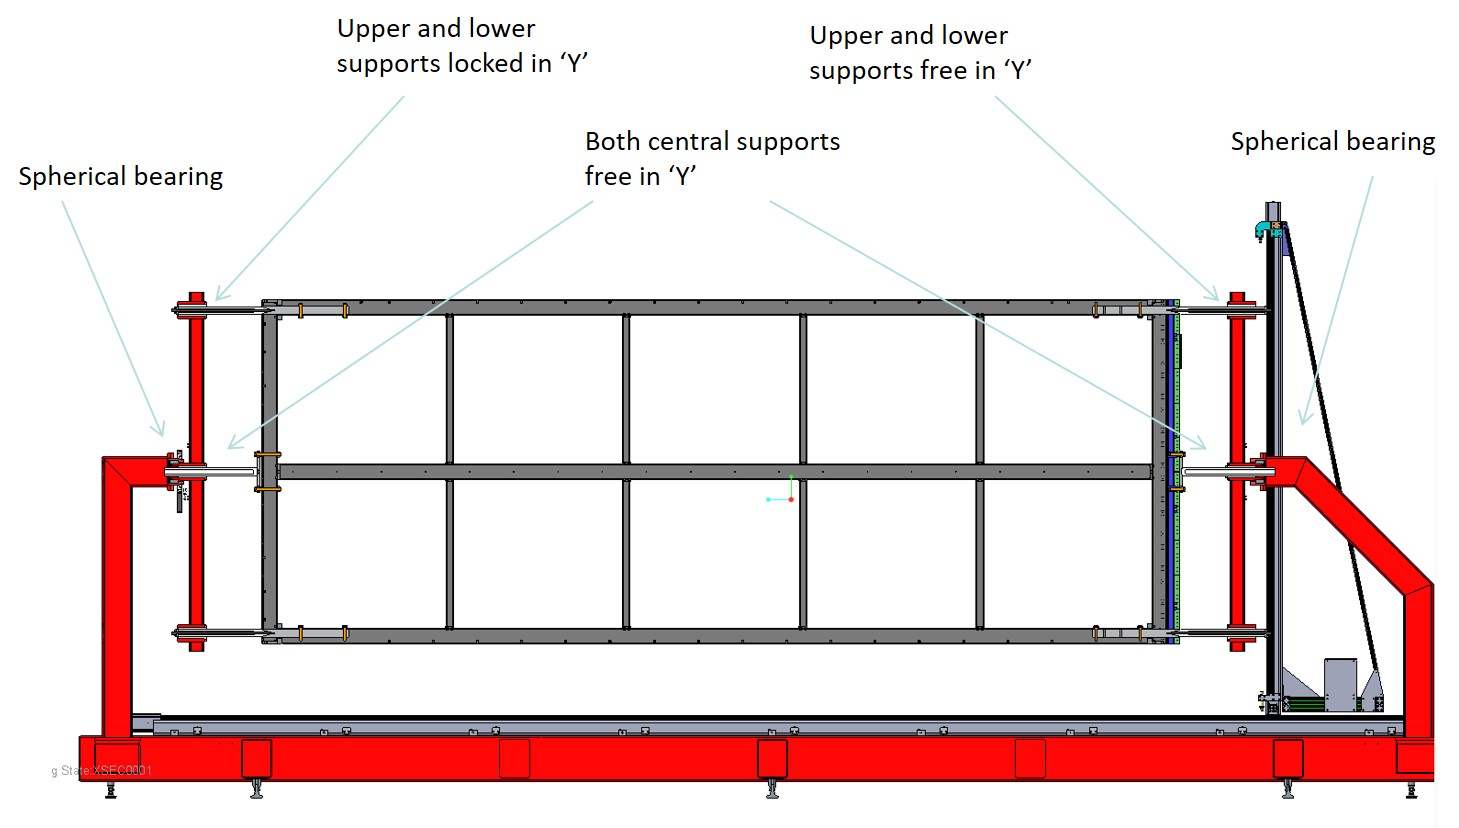
\includegraphics[width=0.95\textwidth]{sp-apa-winding-machine-design-development.jpg} 
\end{dunefigure}

\begin{dunefigure}[APA wire winding machine]{fig:winder-photos}
{Left: Partly wired \dword{pdsp} \dword{apa} on the winding machine at Daresbury Lab, UK. Right: Partly wired \dword{pdsp} \dword{apa} on the winding machine during wire tension measurements at PSL.}
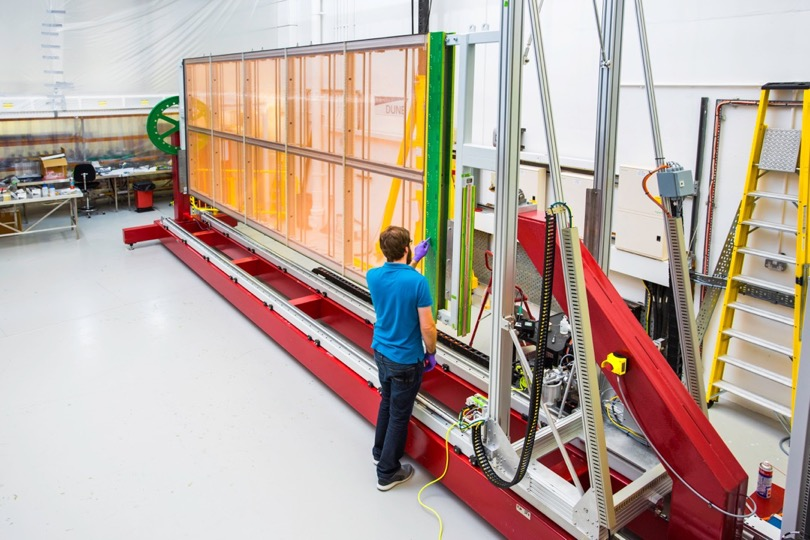
\includegraphics[height=0.3\textheight,trim=25mm 0mm 4mm 0mm,clip]{sp-apa-on-winder-daresbury.jpg}
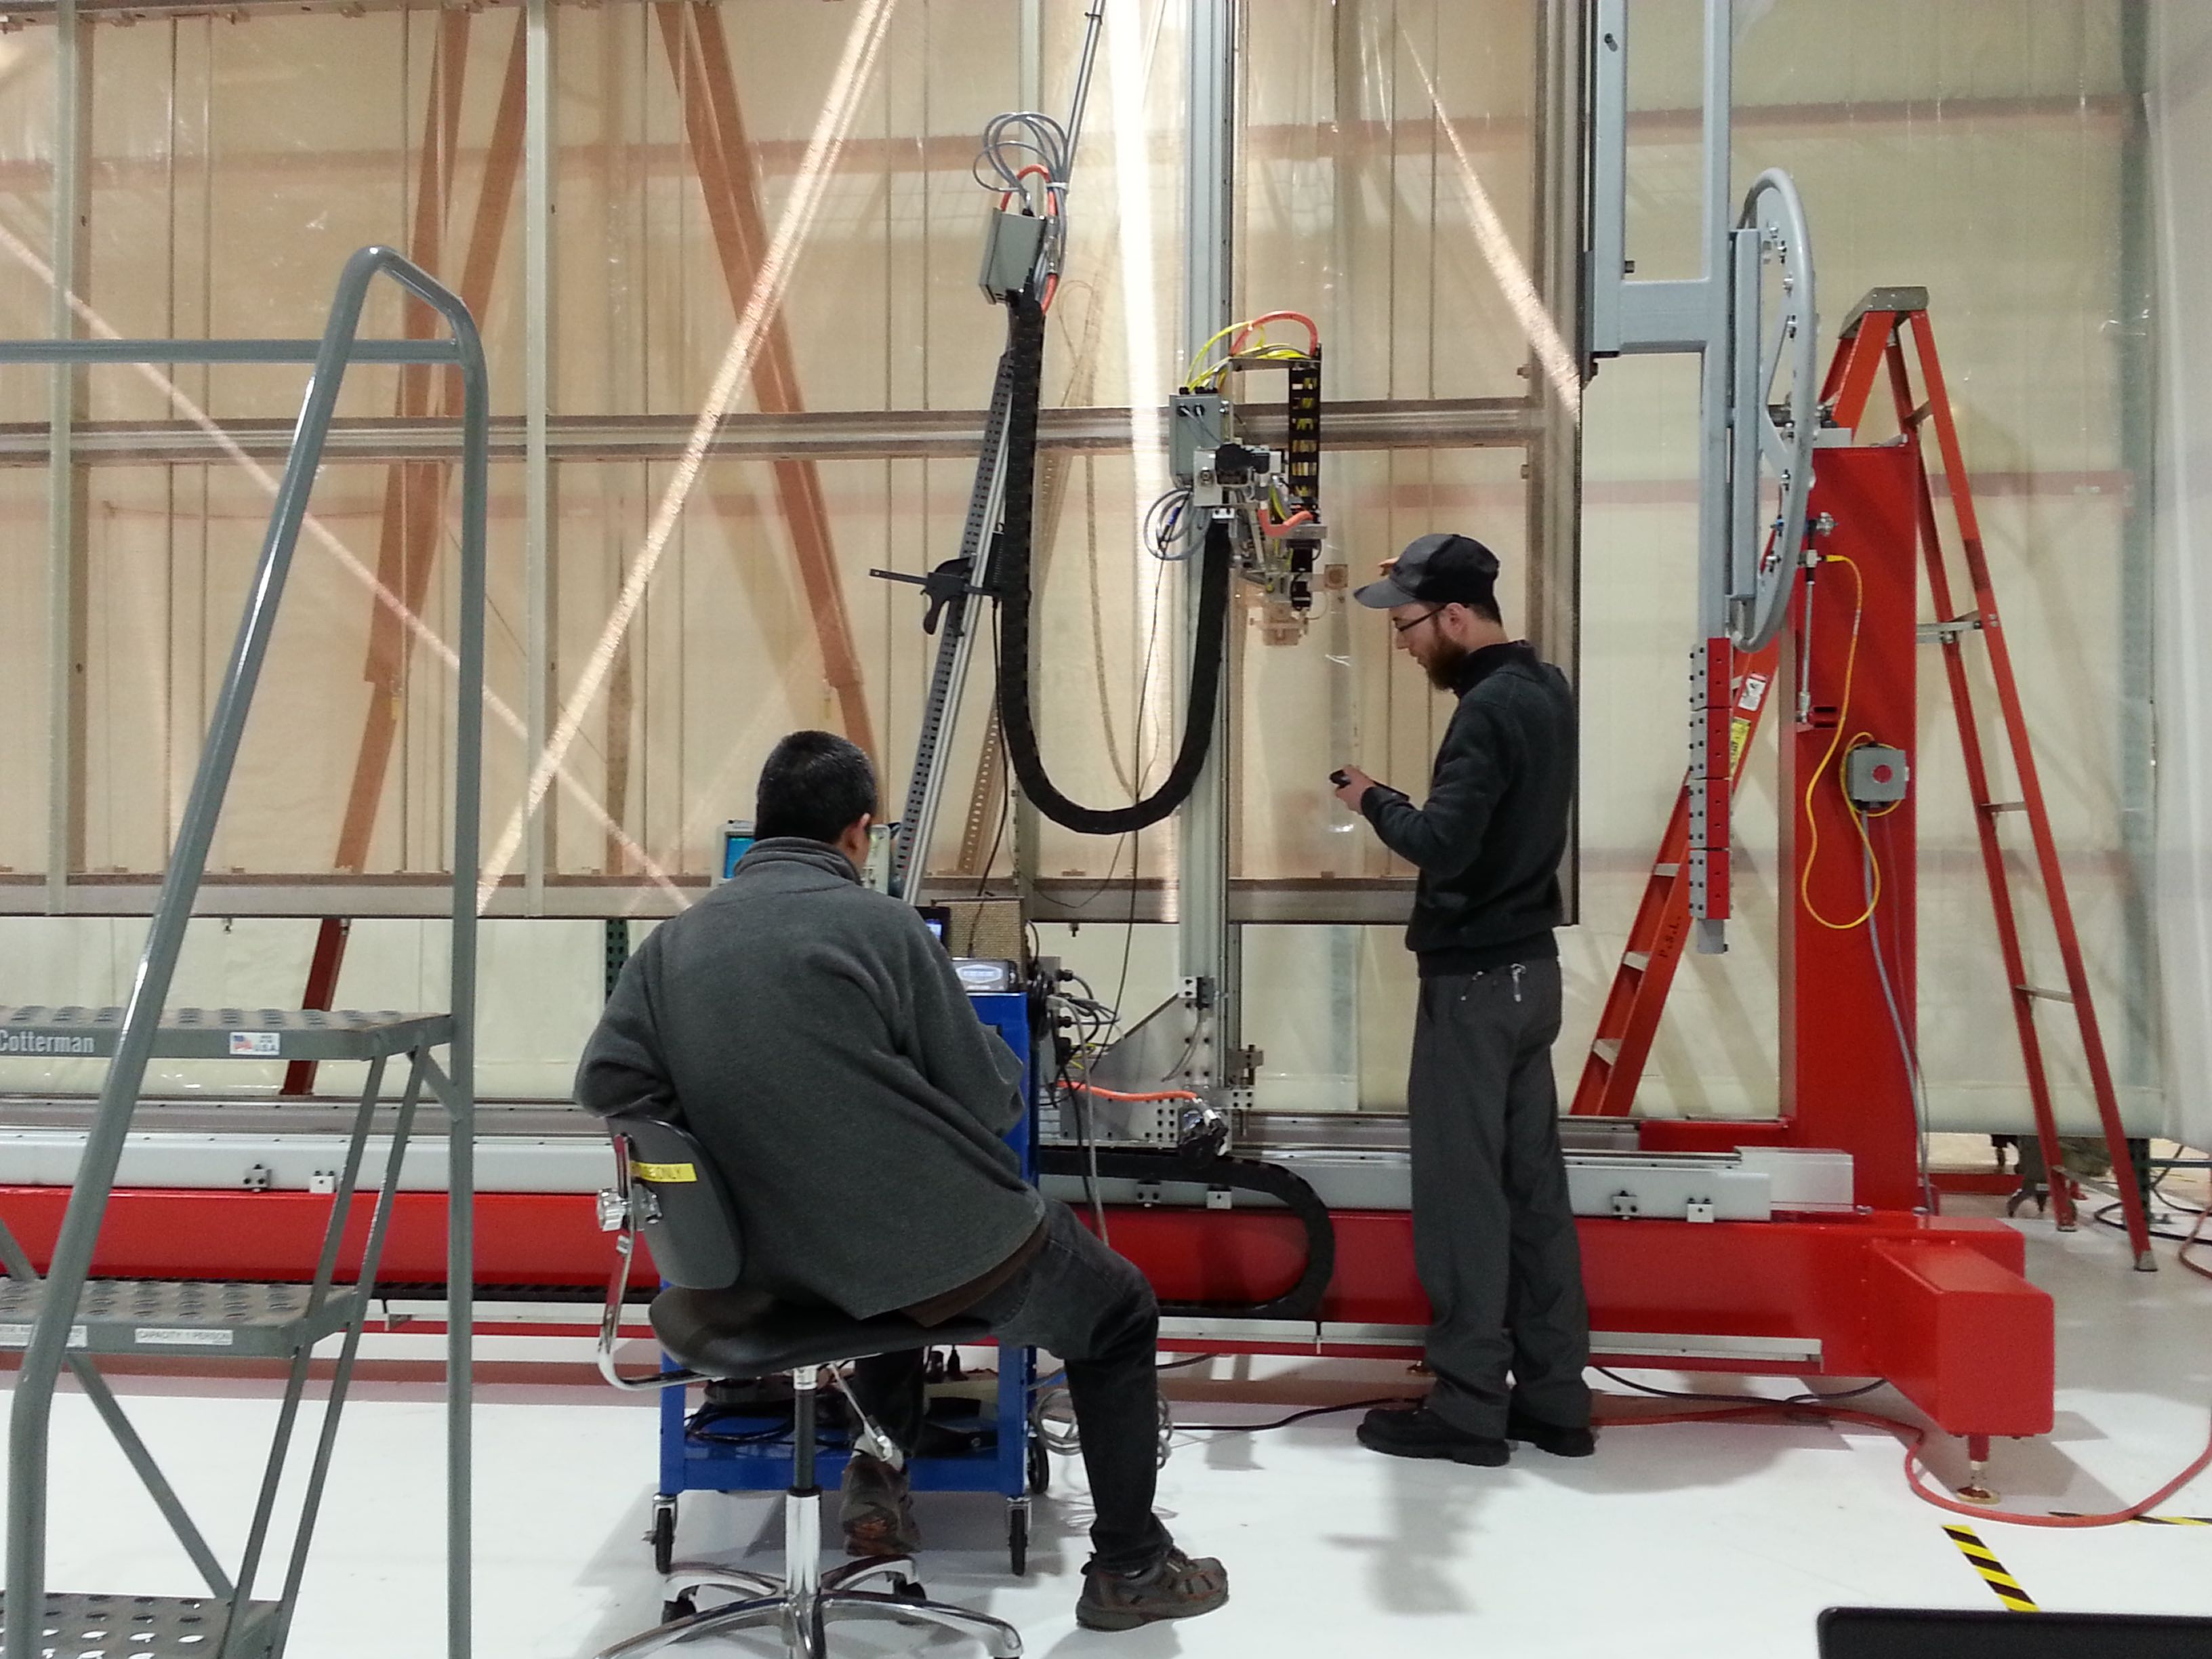
\includegraphics[height=0.3\textheight,trim=200mm 0mm 30mm 0mm,clip]{sp-apa-tension-testing-psl.jpg}
\end{dunefigure}

In the scheme used for \dword{pdsp}, during the winding process, an \dword{apa} moved on and off the winder machine several times for wiring, soldering, and testing, which is time consuming and increases risk.  Several design changes were developed in 2018--2019 to enable the \dword{apa} to remain on the winding machine throughout the wiring process. The design concept allows the winder head to pass from one side to the other nearly continuously. The interface frames at either end have been replaced by retractable linear guided shafts. These can be withdrawn to allow the winding head to pass around the frame over the full height of the frame. These shafts have conical ends and are in shafts fixed to the internal frame tube to provide guides to location. This design change does not alter the design of the frame itself, but it does allow for rotation in the winding machine. Thus, it is now possible to carry out board installation, gluing, and soldering in the winding machine. This eliminates any transfer of the \dword{apa} to the process cart for the entire production operation, which is an inherently safer and faster production method because it cuts down on handling of the \dword{apa}.  The upgraded design has been implemented on the winding machine at Daresbury, which has been used to build a new prototype, APA-07 (see Figure~\ref{fig:winder-upgrade-photos}). All winding, board installation, gluing, soldering and testing operations are being carried out in the winding machine. APA-07 also incorporates the pre-built grounding mesh sub-frames, another new feature since the \dword{pdsp} design that saves significant time in production.  

\begin{dunefigure}[The upgraded APA wire winding machine]{fig:winder-upgrade-photos}
{Left: Upgraded winding machine with new interface arm design being used to wire APA-07. Fitted mesh panels are also shown installed. Right: The V-layer soldering process at the head end of APA-07. Soldering can now be done with the \dword{apa} in the winding machine.}
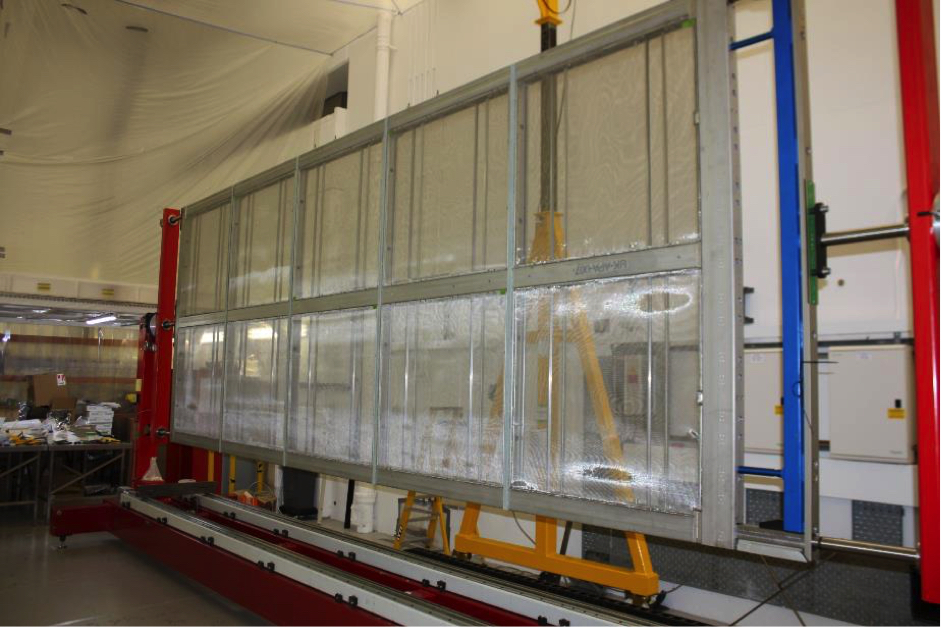
\includegraphics[height=0.25\textheight,trim=10mm 0mm 0mm 0mm,clip]{sp-apa-updated-winder.jpg} 
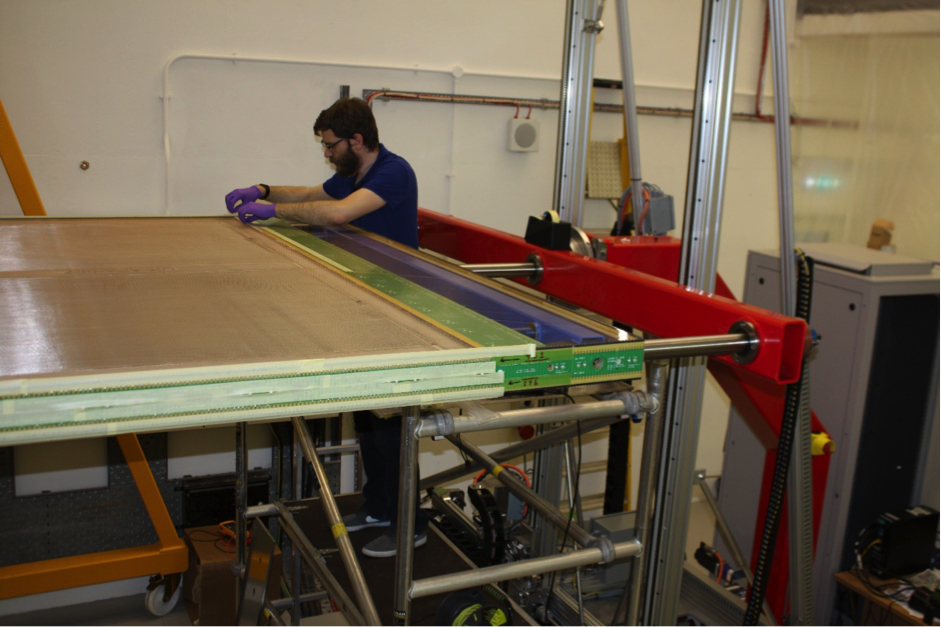
\includegraphics[height=0.25\textheight,trim=0mm 0mm 10mm 0mm,clip]{sp-apa-updated-winder-soldering.jpg}
\end{dunefigure}

Another design effort since \dword{pdsp} construction has been to update the wiring head. The upgraded design offers real-time tension feedback and control, which will enable a big time savings in wiring and produce better tension uniformity across wires.  A prototype of the new head has been constructed and is undergoing extensive commissioning and qualification in 2019.   % and will be tested on a real \dword{apa} soon.     

One important element in the long-term use of the winders for making many \dword{apa}s for \dword{dune} will be maintenance.  The approach to winder maintenance during \dword{pdsp} construction was not well considered. As a result, winding machine problems traceable to lack of routine maintenance occurred from time to time, shutting the production line down until repair or maintenance was performed. We will formulate a routine and preventive maintenance plan that minimizes winder downtime during \dword{apa} production.

Another key element in the flow of activities during production are large process carts, with an example shown in Figure~\ref{fig:apa-process-cart}. The process carts can be used to hold \dword{apa}s during wiring preparations and for quality control checks after wiring and to safely move \dword{apa}s around within the assembly facility. Process carts are fitted with specialized 360$^\circ$ rotating casters that allow the cart, loaded with a fully assembled \dword{apa}, to maneuver corners while moving the large frames between preparation, assembly, and packing/shipping areas.

\begin{dunefigure}[APA on a process cart during construction]{fig:apa-process-cart}
{A \dword{pdsp} \dword{apa} being moved around the PSL production facility on a process cart.}
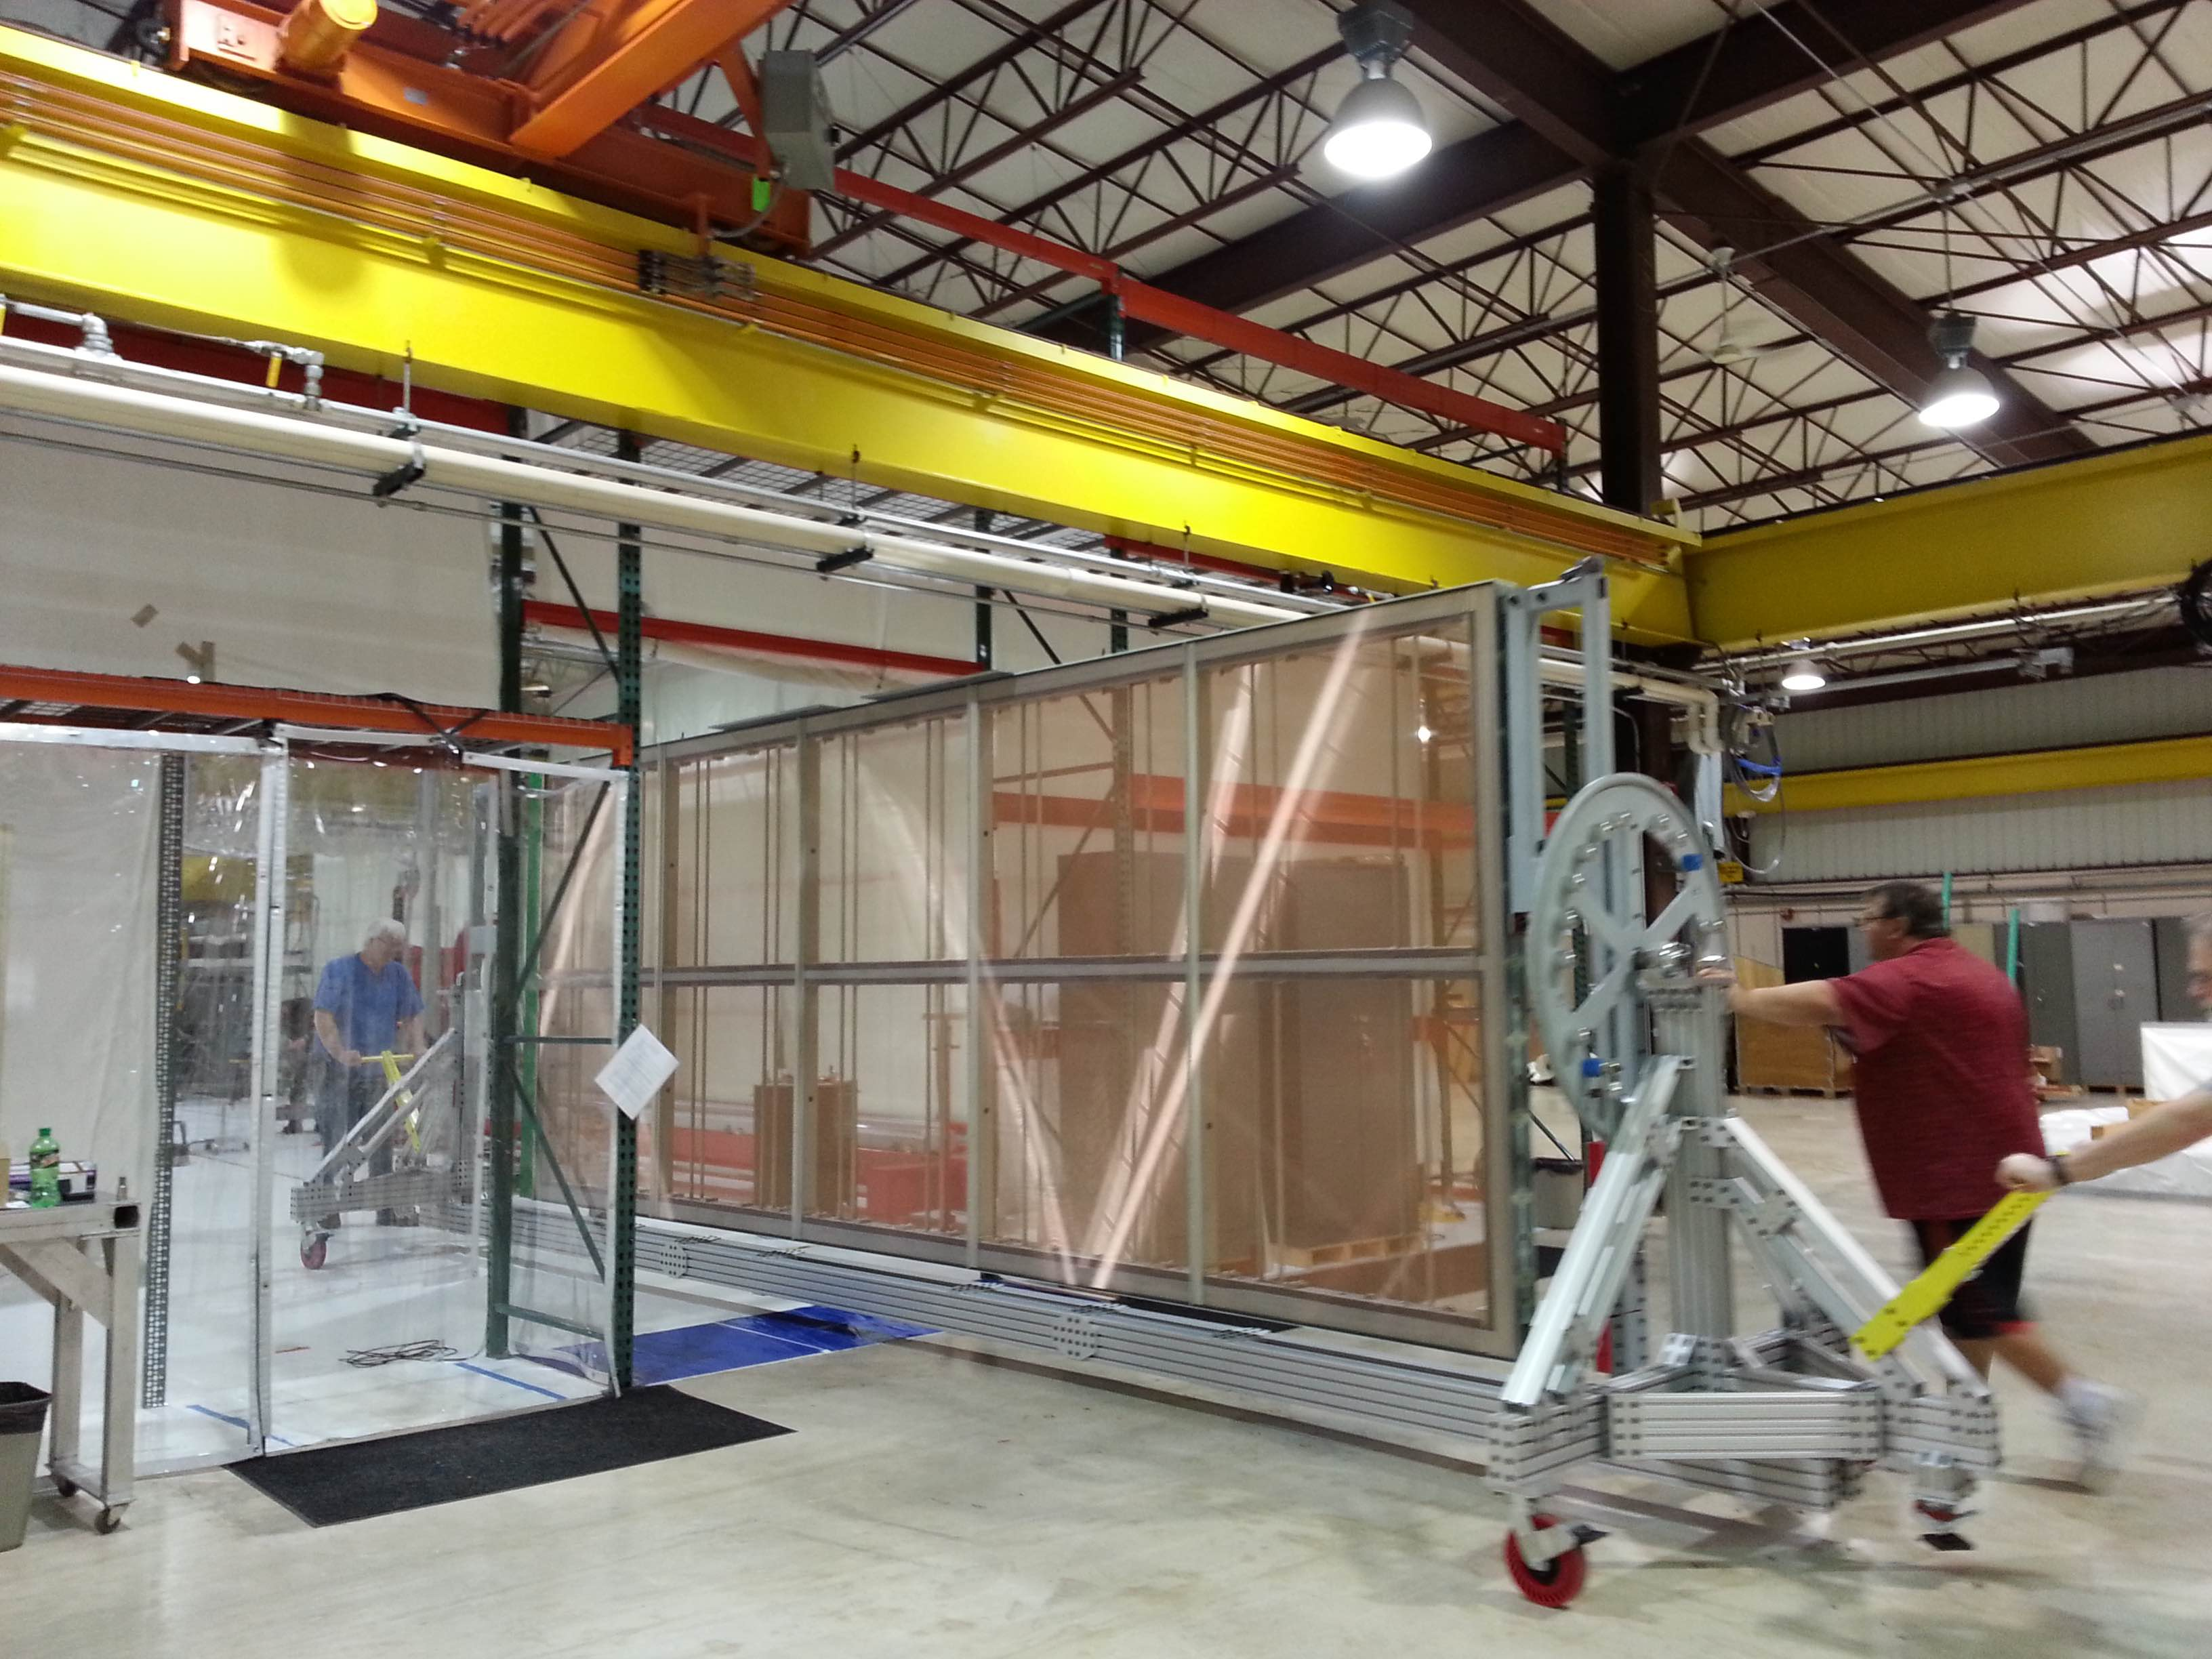
\includegraphics[height=0.35\textheight,trim=50mm 10mm 70mm 250mm,clip]{sp-apa-process-cart.jpg}
\end{dunefigure}

%Before wiring can begin, the grounding mesh panels must be installed on the bare frame. 
%
%In the \dword{pdsp} design, a large jig holds the mesh in place for gluing. Once the jig is sufficiently leveled to the frame, a mesh sheet is laid into place and hold down bars are iteratively moved and repositioned until the mesh is flat and tight.  The outside edge of the mesh panel is then epoxied, and the jig and hold down bars remain in place for a 12 hour epoxy cure cycle.  This process is then repeated for the next three shifts until all four panels of mesh have been attached to the bare \dword{apa} frame.  As described below, we are considering changes to this lengthy procedure for DUNE \dwords{apa}.  

%Another custom construction jig is needed to install the wire combs that hold the wires at intermediate points above the four cross beams of the \dword{apa}.  Currently, two jigs can be loaded and installed at a time, and each installation requires a six-hour epoxy cure cycle. %the two jigs are removed from the initial locations and placed in another two locations, on the same side of the \dword{apa}.  Thus four comb bases are installed within one operation shift and the \dword{apa} is left in this horizontal position to cure overnight.  The next day, the \dword{apa} is flipped to the reverse side and the process is repeated for the other side. Figure~\ref{fig:apa-process-cart} shows the comb installation jig in use.  

%\subsubsection{Planned Improvements to Production Process}


%Another area for potential improvement in the construction process that could make \dword{apa} fabrication more efficient and reliable is the technique used to measure wire tensions.  Individual wire tension can be determined by measuring the resonant vibration frequency of a wire that has been mechanically disturbed.  The current technique involves manually plucking the wires and using a laser photodiode tool mounted on the winder to measure tension one wire at a time.  This takes many hours for each wire plane. A task force within the consortium was recently initiated to study the problem and consider possible new approaches to measuring tension. In particular, methods to electronically disturb and measure groups of \num{20} or more wires at one time have recently been explored, so the task force is studying the feasibility of applying this during \dword{apa} construction. The recent developments, where an electronics board has been designed to supply the voltages to multiple wires while reading out the resonance frequency of vibration of the measured wires, have shown promising results. Scanning the wire tension of a full wire plane should take only a few minutes. Further tests and studies are required to validate the electrical methods, and a final prototype should be available soon. With such a less labor intensive and faster method, it also becomes possible to measure more of the wire tensions later in the construction of the detector, for example during integration and installation at \dword{surf}.  


%\begin{itemize}

%\item Wiring head design: Efforts to improve winder head performance are already underway. We envision improved tension control, continuous tension feedback, improved clutch, and improvement to the compensator mechanism, all leading to better, more consistent, and more reliable winder performance.  The current winding head uses a magnetic clutch mechanism that is manually adjusted to increase or decrease the tension of the wire as it is wound around the \dword{apa}. The clutch regularly needs adjustment because the diameter of the wire on the spool declines during the winding process. In addition, if the mechanism is run from a cold start, the tension changes after $\sim$10 minutes of running. Experience winding the \dword{pdsp} \dwords{apa} has shown that maintaining the target tension within tolerances (5$\pm$\SI{1}{N} for \dword{pdsp}) is difficult.

%A solution to this issue is to design a winder head with active tension control by replacing the magnetic clutch with a servo motor and introducing a potentiometer on a dancer arm for the feedback loop (see Figure~\ref{fig:winding-head}). This only works if no signal losses occur when transferring the winding head to the compensator latching mechanism and back. The system can be driven in torque mode and should compensate for any wire spool changes. It must be able to operate from a cold start. This development is well underway, and the changes are being tested.

%\begin{dunefigure}[Exploded view of the winding machine head]{fig:winding-head}
%{Exploded view of winder head with active tension control.}
%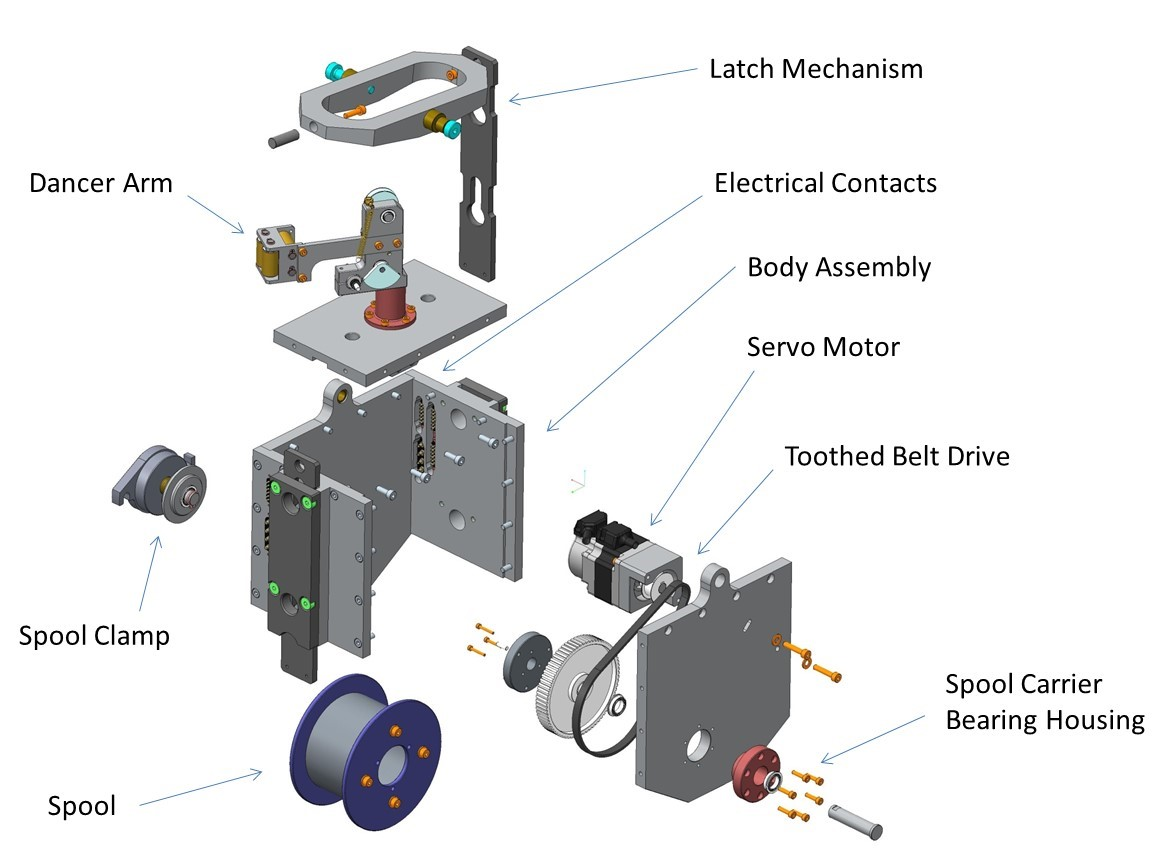
\includegraphics[width=0.7\textwidth]{sp-apa-winder-head-with-active-tension-controls.jpg}
%\end{dunefigure}

%\item Winder interface arm design: The current winder interface only allows one-half of a wire plane to be wired at a time. The \dword{apa} frame must be moved to the process cart where the interface arms are flipped 180$^\circ$ to wind the second half of the wire plane.  A new design concept, illustrated in Figure~\ref{fig:winding-dev}, allows the winder head to pass from one side to the other nearly continuously without removing the frame from the winding machine.  The interface frames are replaced at either end by retractable linear guided shafts. These can be withdrawn to allow the winding head to pass around the frame over the full height of the frame. These shafts have conical ends and are in shafts fixed to the internal frame tube to provide guides to location. This design change does not alter the design of the frame itself, but it does allow for rotation in the winding machine. Thus, it should also be possible to carry out board installation, gluing, and soldering in the winding machine. This eliminates any transfer of the \dword{apa} to the process cart for the entire production operation, which is an inherently safer and faster production method because it cuts down on handling the \dword{apa}.

%\item Modular mesh panels: The current approach to mesh installation is slow and cumbersome. We will improve this part of construction by moving toward a modular window screen design that improves the reliability of the installed mesh (more uniform tension across the mesh) and allows much easier installation on the \dword{apa} frame.

%\fixme{Can you please check the following paragraph? I was interrupted while working on it, and I'm afraid it's not accurate any more.}

%\item Epoxy process improvements: Applying epoxy during the construction process requires many steps. These steps require careful work and many hours between winding each successive wire plane as the epoxy cures. We already have concepts for improving epoxy application jigs from \dword{pdsp}, and we will investigate whether epoxy pre-forms or accelerated heat curing can improve time or reliability.

%\item Automated soldering: Every solder joint on the six \dword{pdsp} \dwords{apa} was done by hand. We will investigate automated soldering techniques to improve the process and reduce the amount of manual effort required. 

%\item Wire tension measurement techniques: Verifying wire tension during construction is an important, but time consuming, process. The current technique uses a laser photodiode tool mounted on the winder to measure tension one wire at a time. This takes many hours for each wire plane. Collaborators at the University of Manchester are developing techniques to electronically measure groups of \num{20} or more wires at one time. This technique provides much faster tension measurements and shorter turnaround between wire planes. 

%\item Winder maintenance plan: The approach to winder maintenance during \dword{pdsp} construction was not well considered. As a result, winding machine problems traceable to lack of routine maintenance occurred from time to time, shutting the production line down until repair or maintenance was performed. We will formulate a routine and preventive maintenance plan that minimizes winder downtime during \dword{apa} production.
%\end{itemize}


%%%%%%%%%%%%%%%%%%%%%%%%%%%%%%%%%%%%%%%%%%%%%%%%%%%%%%%%%%%%%%%%%%%%%%%%%%%
\subsection{APA Production Sites}
\label{sec:fdsp-apa-prod-facility}
%%%%%%%%%%%%%%%%%%%%%%%%%%%%%%%%%%%%%%%%%%%%%%%%%%%%%%%%%%%%%%%%%%%%%%%%%%%

Construction of \dword{spmod} \dwords{apa} will take place in both the USA and the UK.  Multiple \dword{apa} production lines spread over several sites will provide some margin on the production schedule and provide backup in the event that technical problems occur at any particular site. 

The space requirements for each production line are driven by the size of the \dword{apa} frames and the winding robot used to build them. The approximate dimensions of a class \num{100000} clean space needed to house winder operations and associated tooling is \SI{175}{m$^2$}. The estimated requirement for inventory, work in progress, and completed \dwords{apa} is about \SI{600}{m$^2$}. Each facility  also needs temporary access to shipping and crating space of about \SI{200}{m$^2$}. Floor layouts at each institution are being developed, with current layouts shown in Figure~\ref{fig:factories}. Adequate space is available at each site, and the institutions have offered commitments for space for \dword{dune}. 

At Daresbury Laboratory in the UK, the existing single production line used for \dword{pdsp} construction will be expanded to four.  The Inner Hall on the Daresbury site has been identified as an area that is large enough to be used for \dword{dune} \dword{apa} construction. It has good access and crane coverage throughout. Daresbury Laboratory management have agreed that the area is available, and a working environment that meets \dword{dune}'s safety standards is now being prepared, starting with clearing the current area of existing facilities, obsolete cranes, and ancillary equipment. The renovation of a plant room is also ongoing, so it can be used for storage and as a shipping area. The production area is designed to hold four winding machines and associated process equipment and tooling.  A production site design review of the Daresbury facility is planned for October 2019, and a production site readiness review is anticipated for June 2020, followed by the start of \dword{apa} production for \dword{dune} \dword{detmodule} \#1 in August 2020.  

\begin{dunefigure}[Layouts of APA production sites]{fig:factories}
{Developing concepts for production site layouts at Daresbury Lab (top left), University of Chicago (top right), and Yale University (bottom left), and the existing APA production area at PSL (bottom right).}
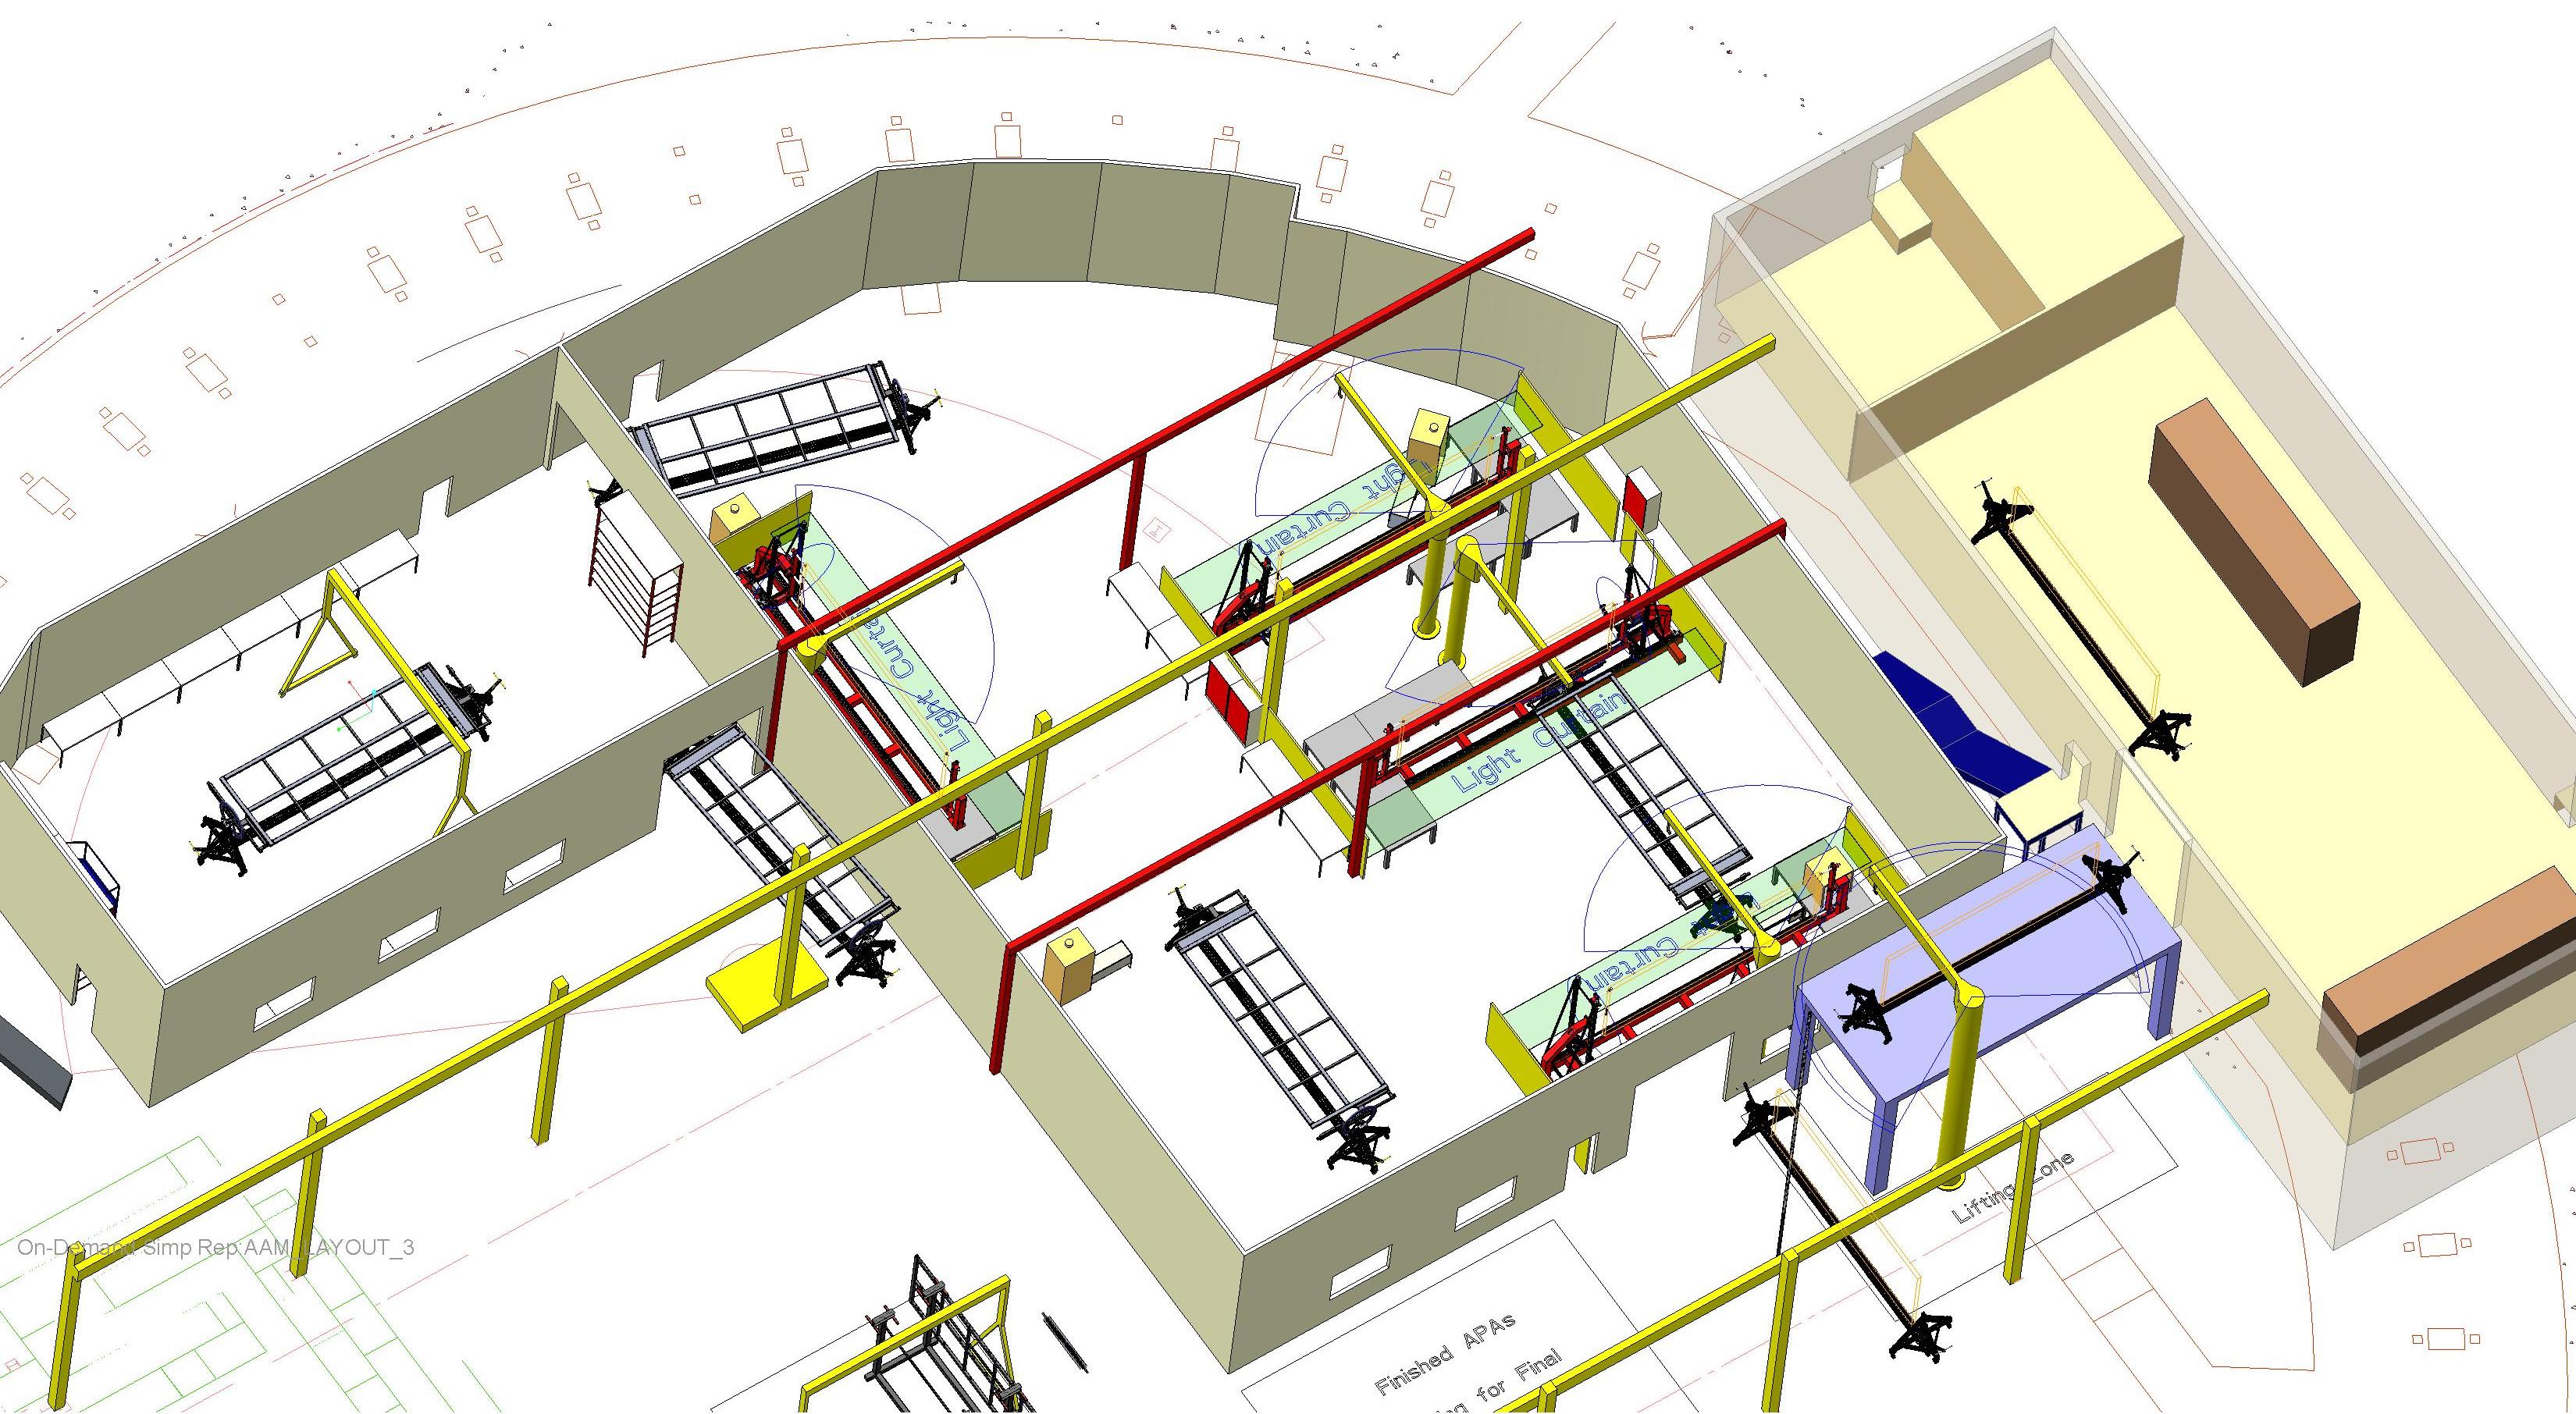
\includegraphics[height=0.23\textheight]{sp-apa-factory-daresbury.jpg} 
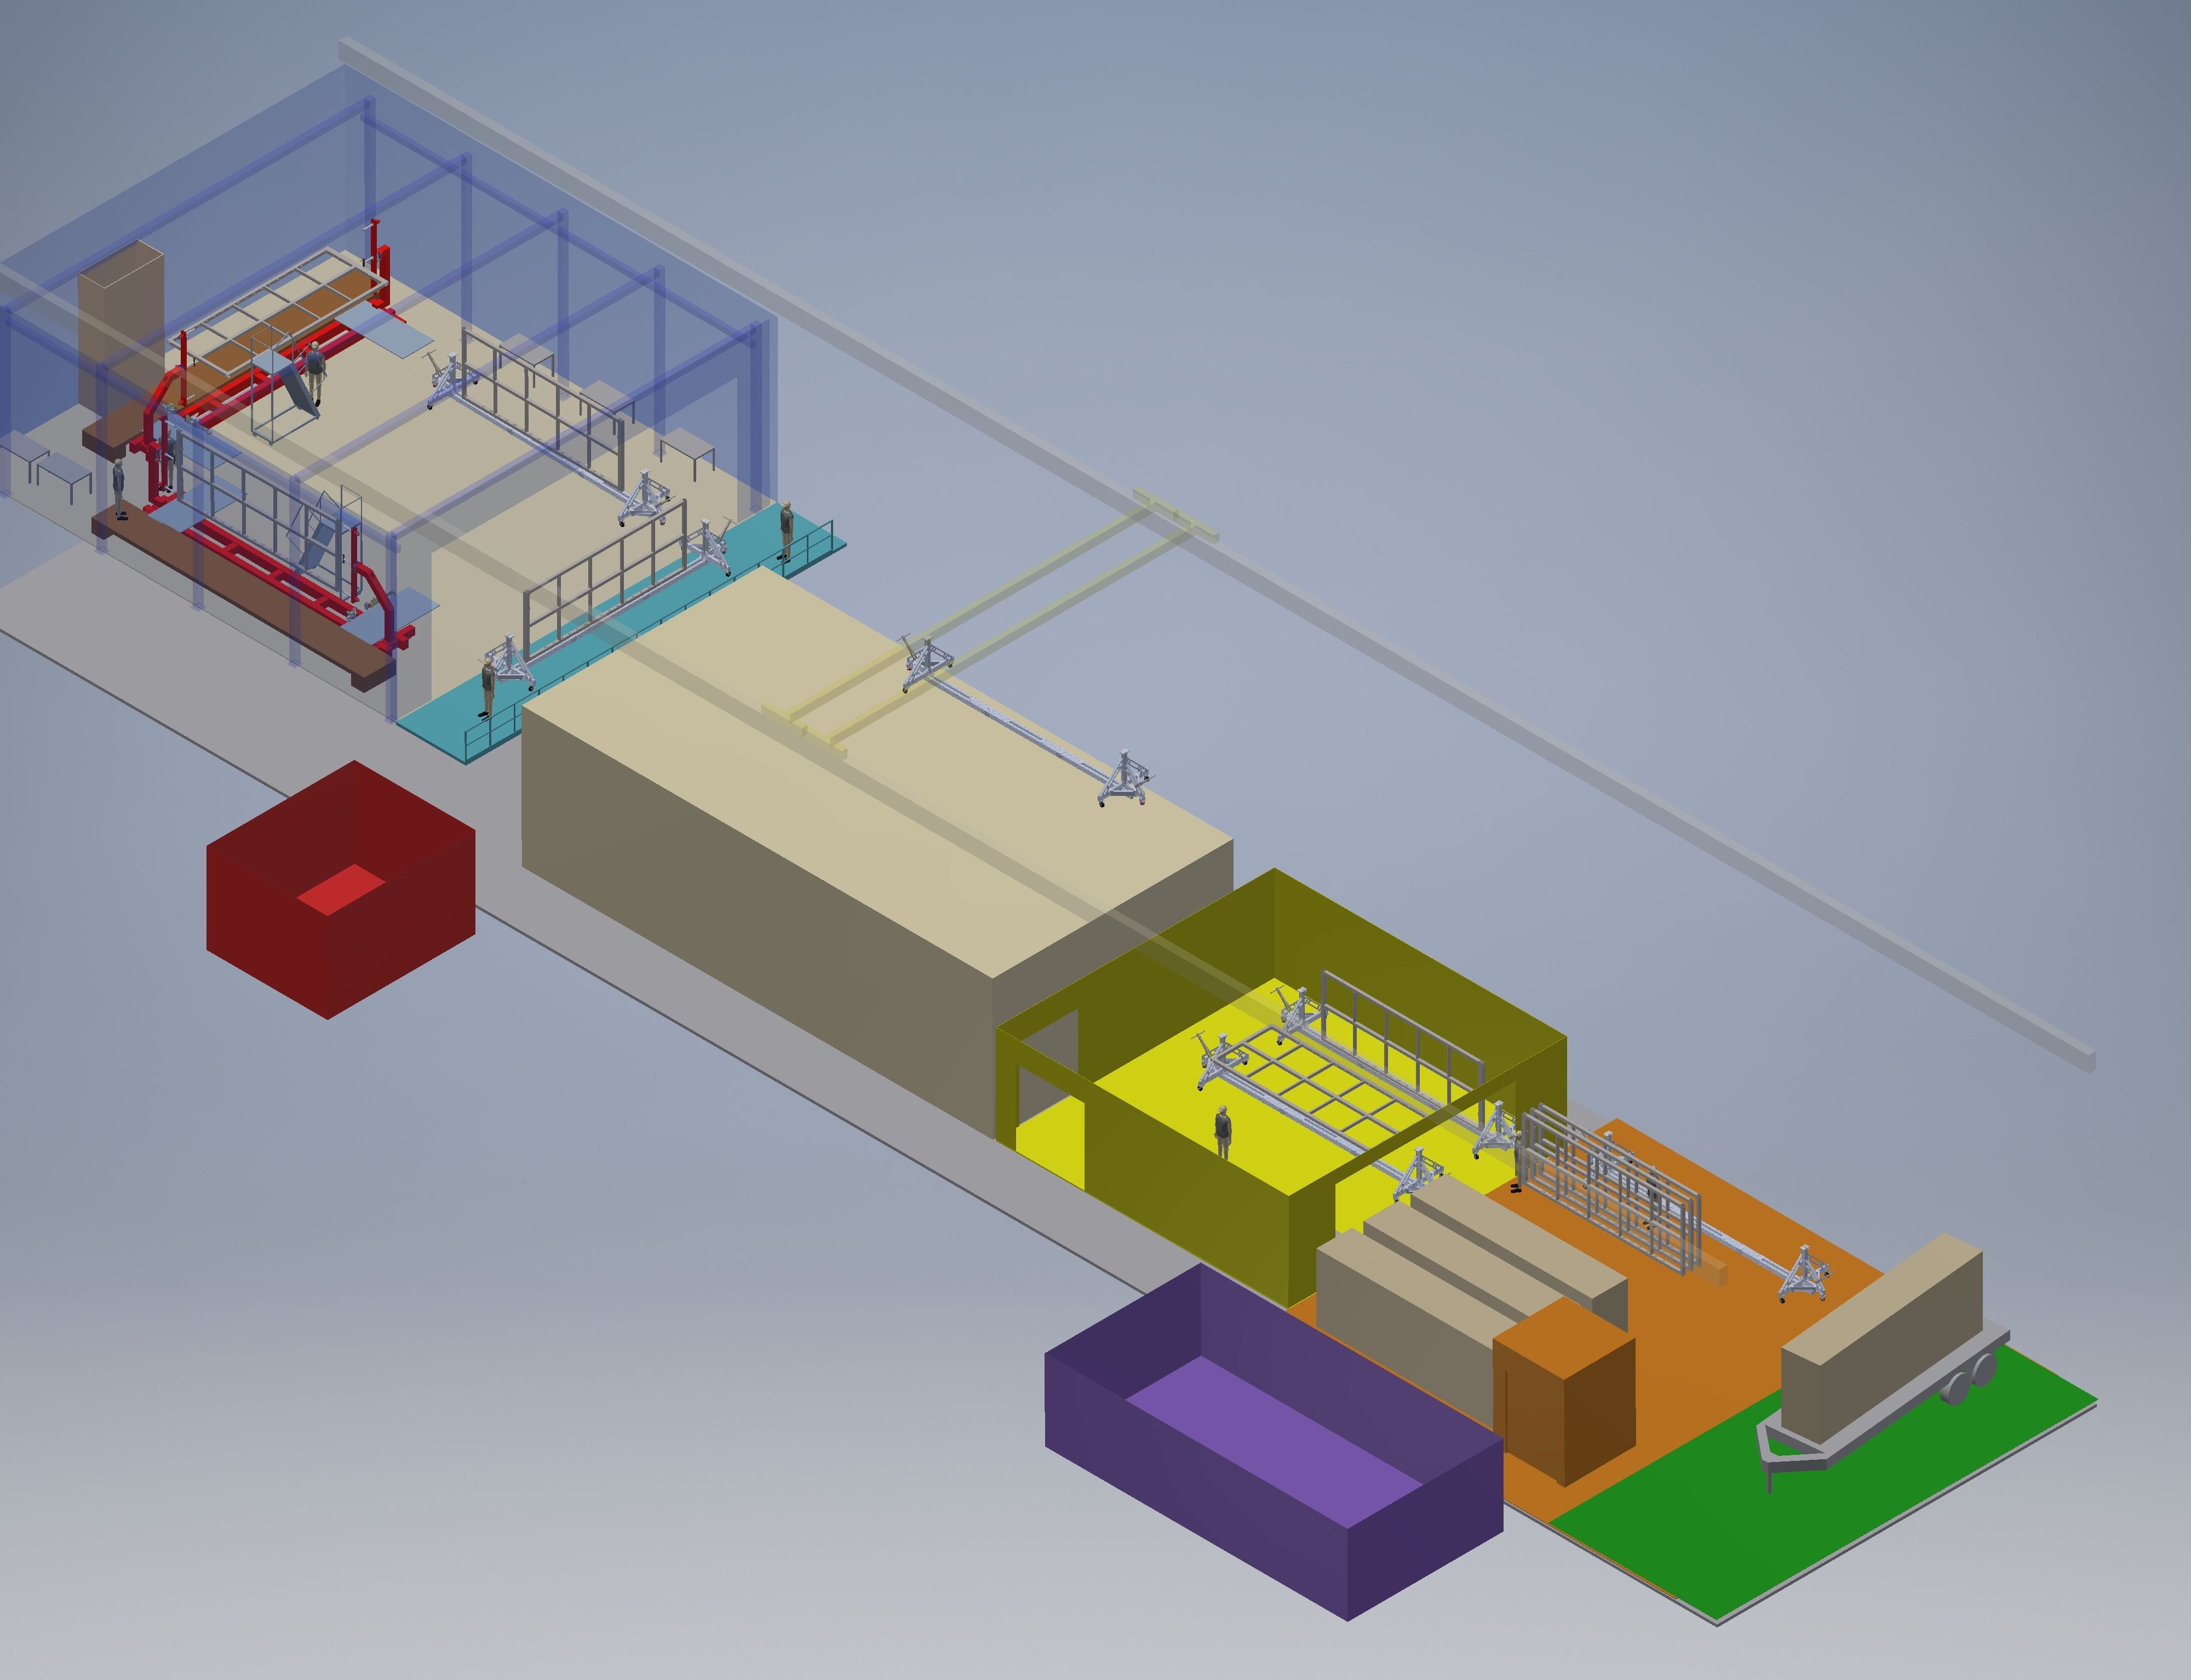
\includegraphics[height=0.23\textheight]{sp-apa-factory-chicago.jpg} \\
\vspace{1mm}
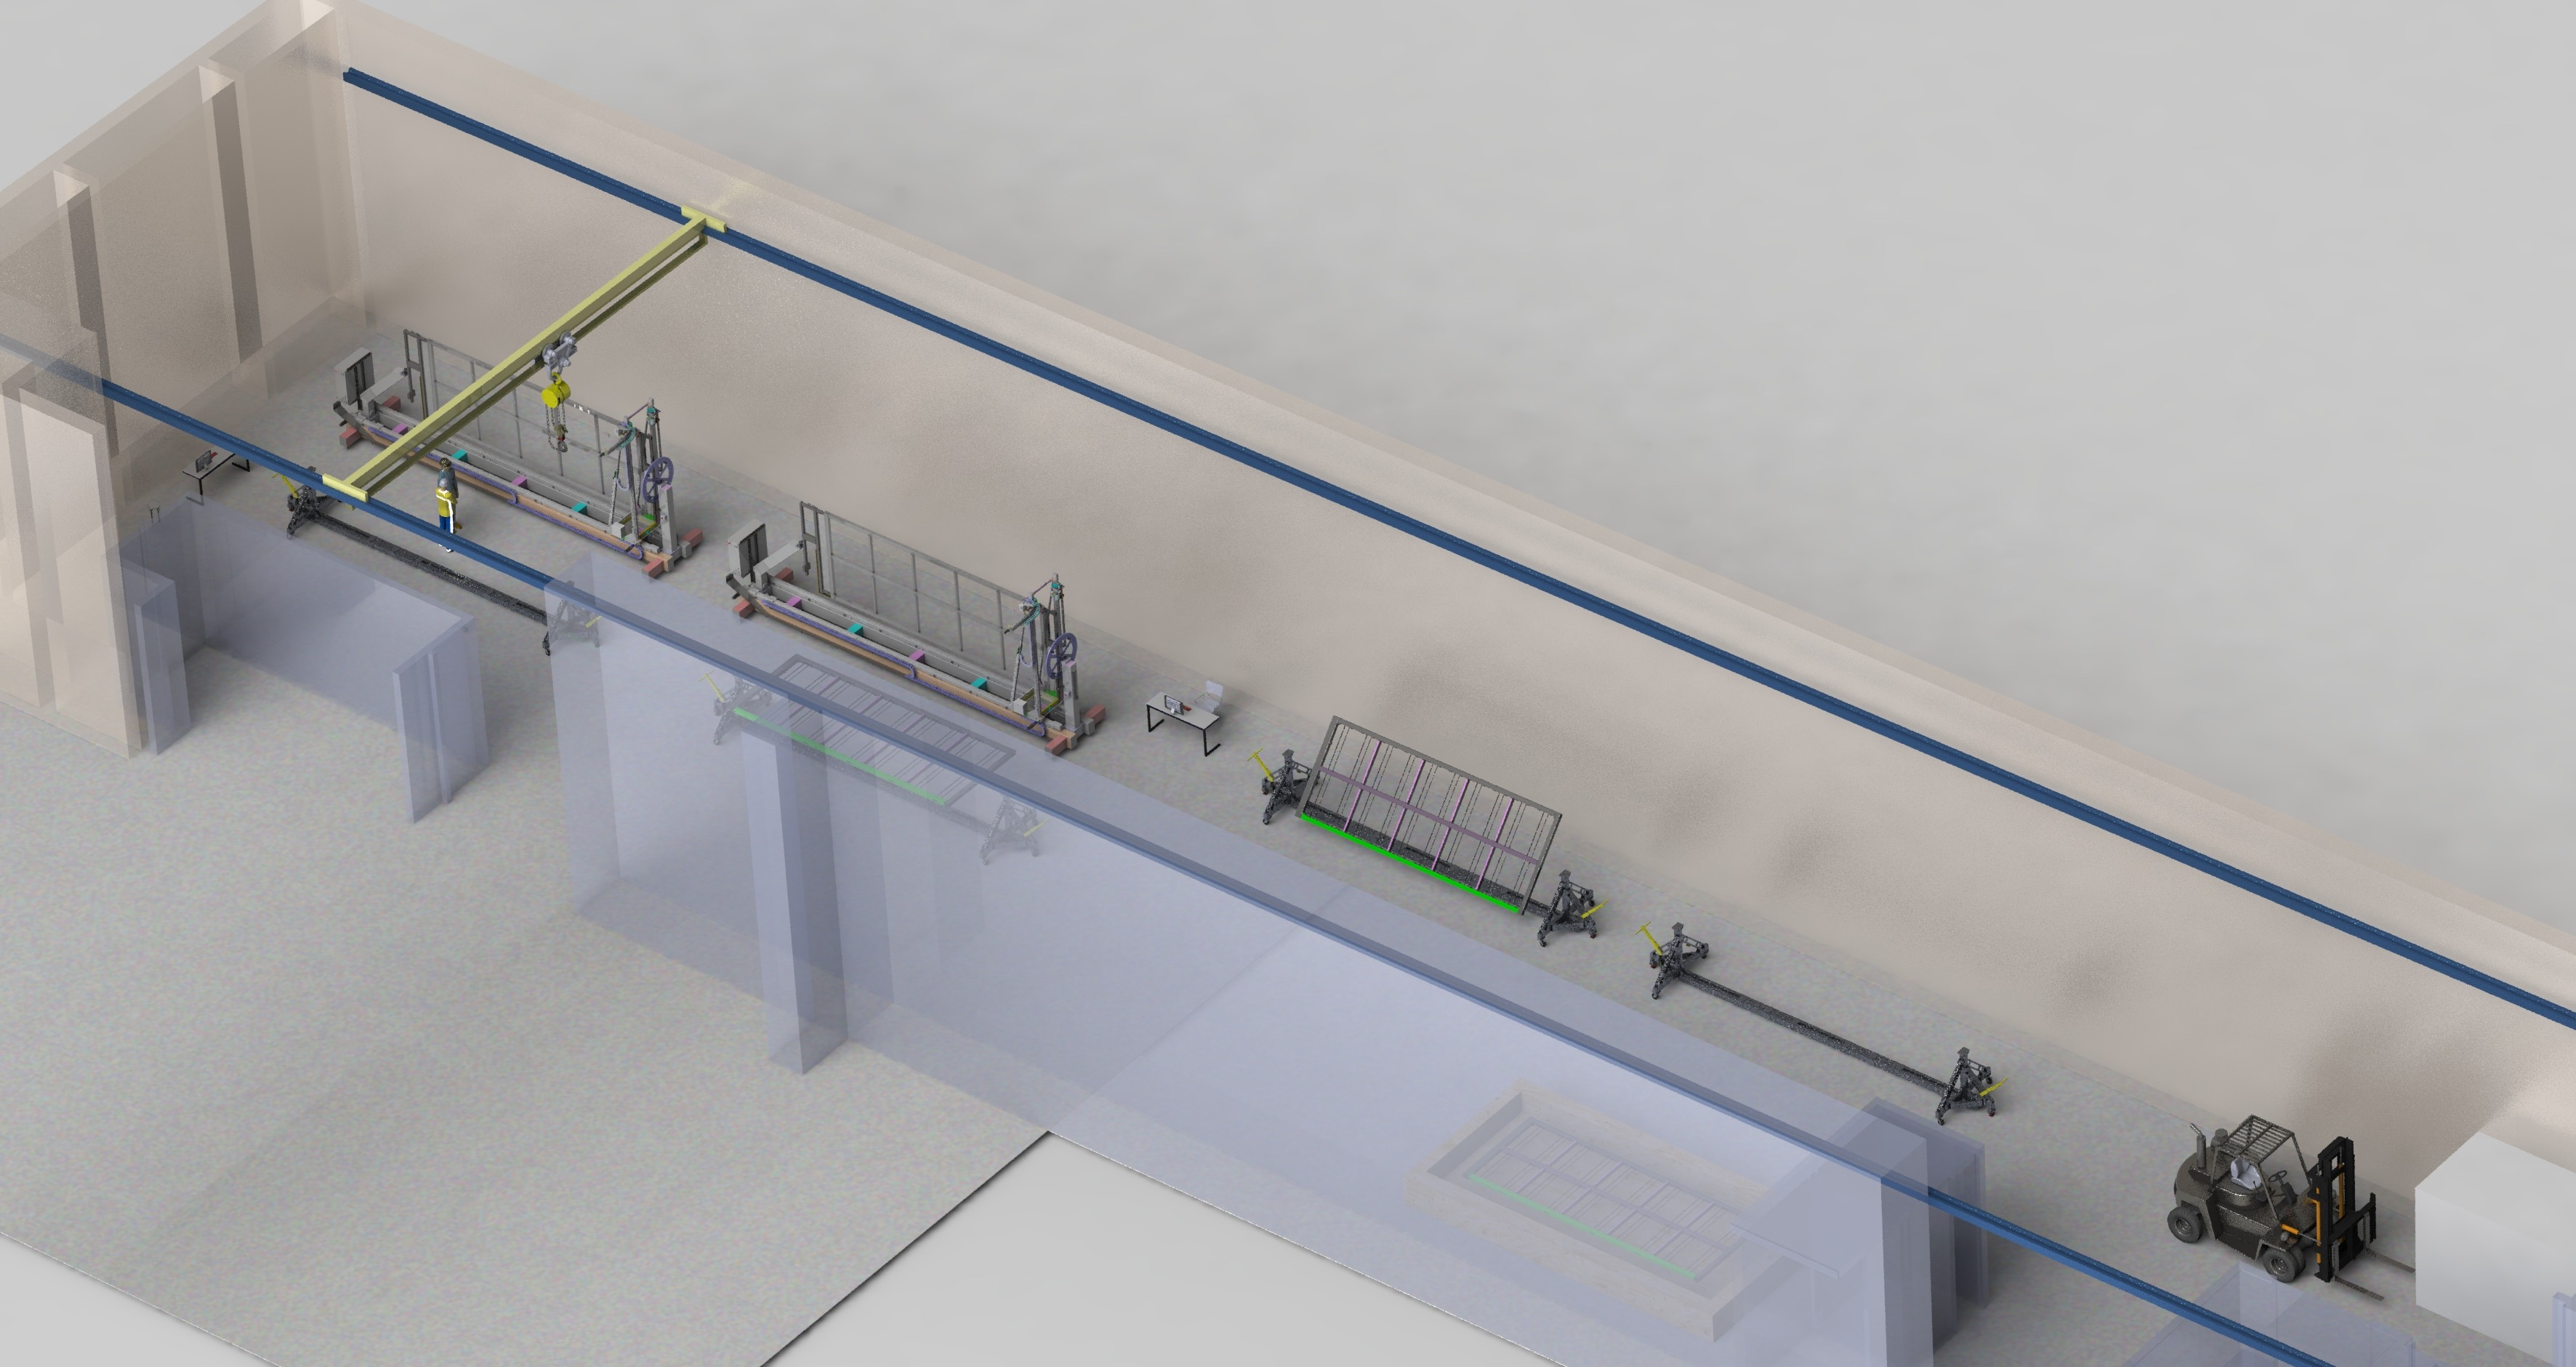
\includegraphics[height=0.225\textheight]{sp-apa-factory-yale.jpg}
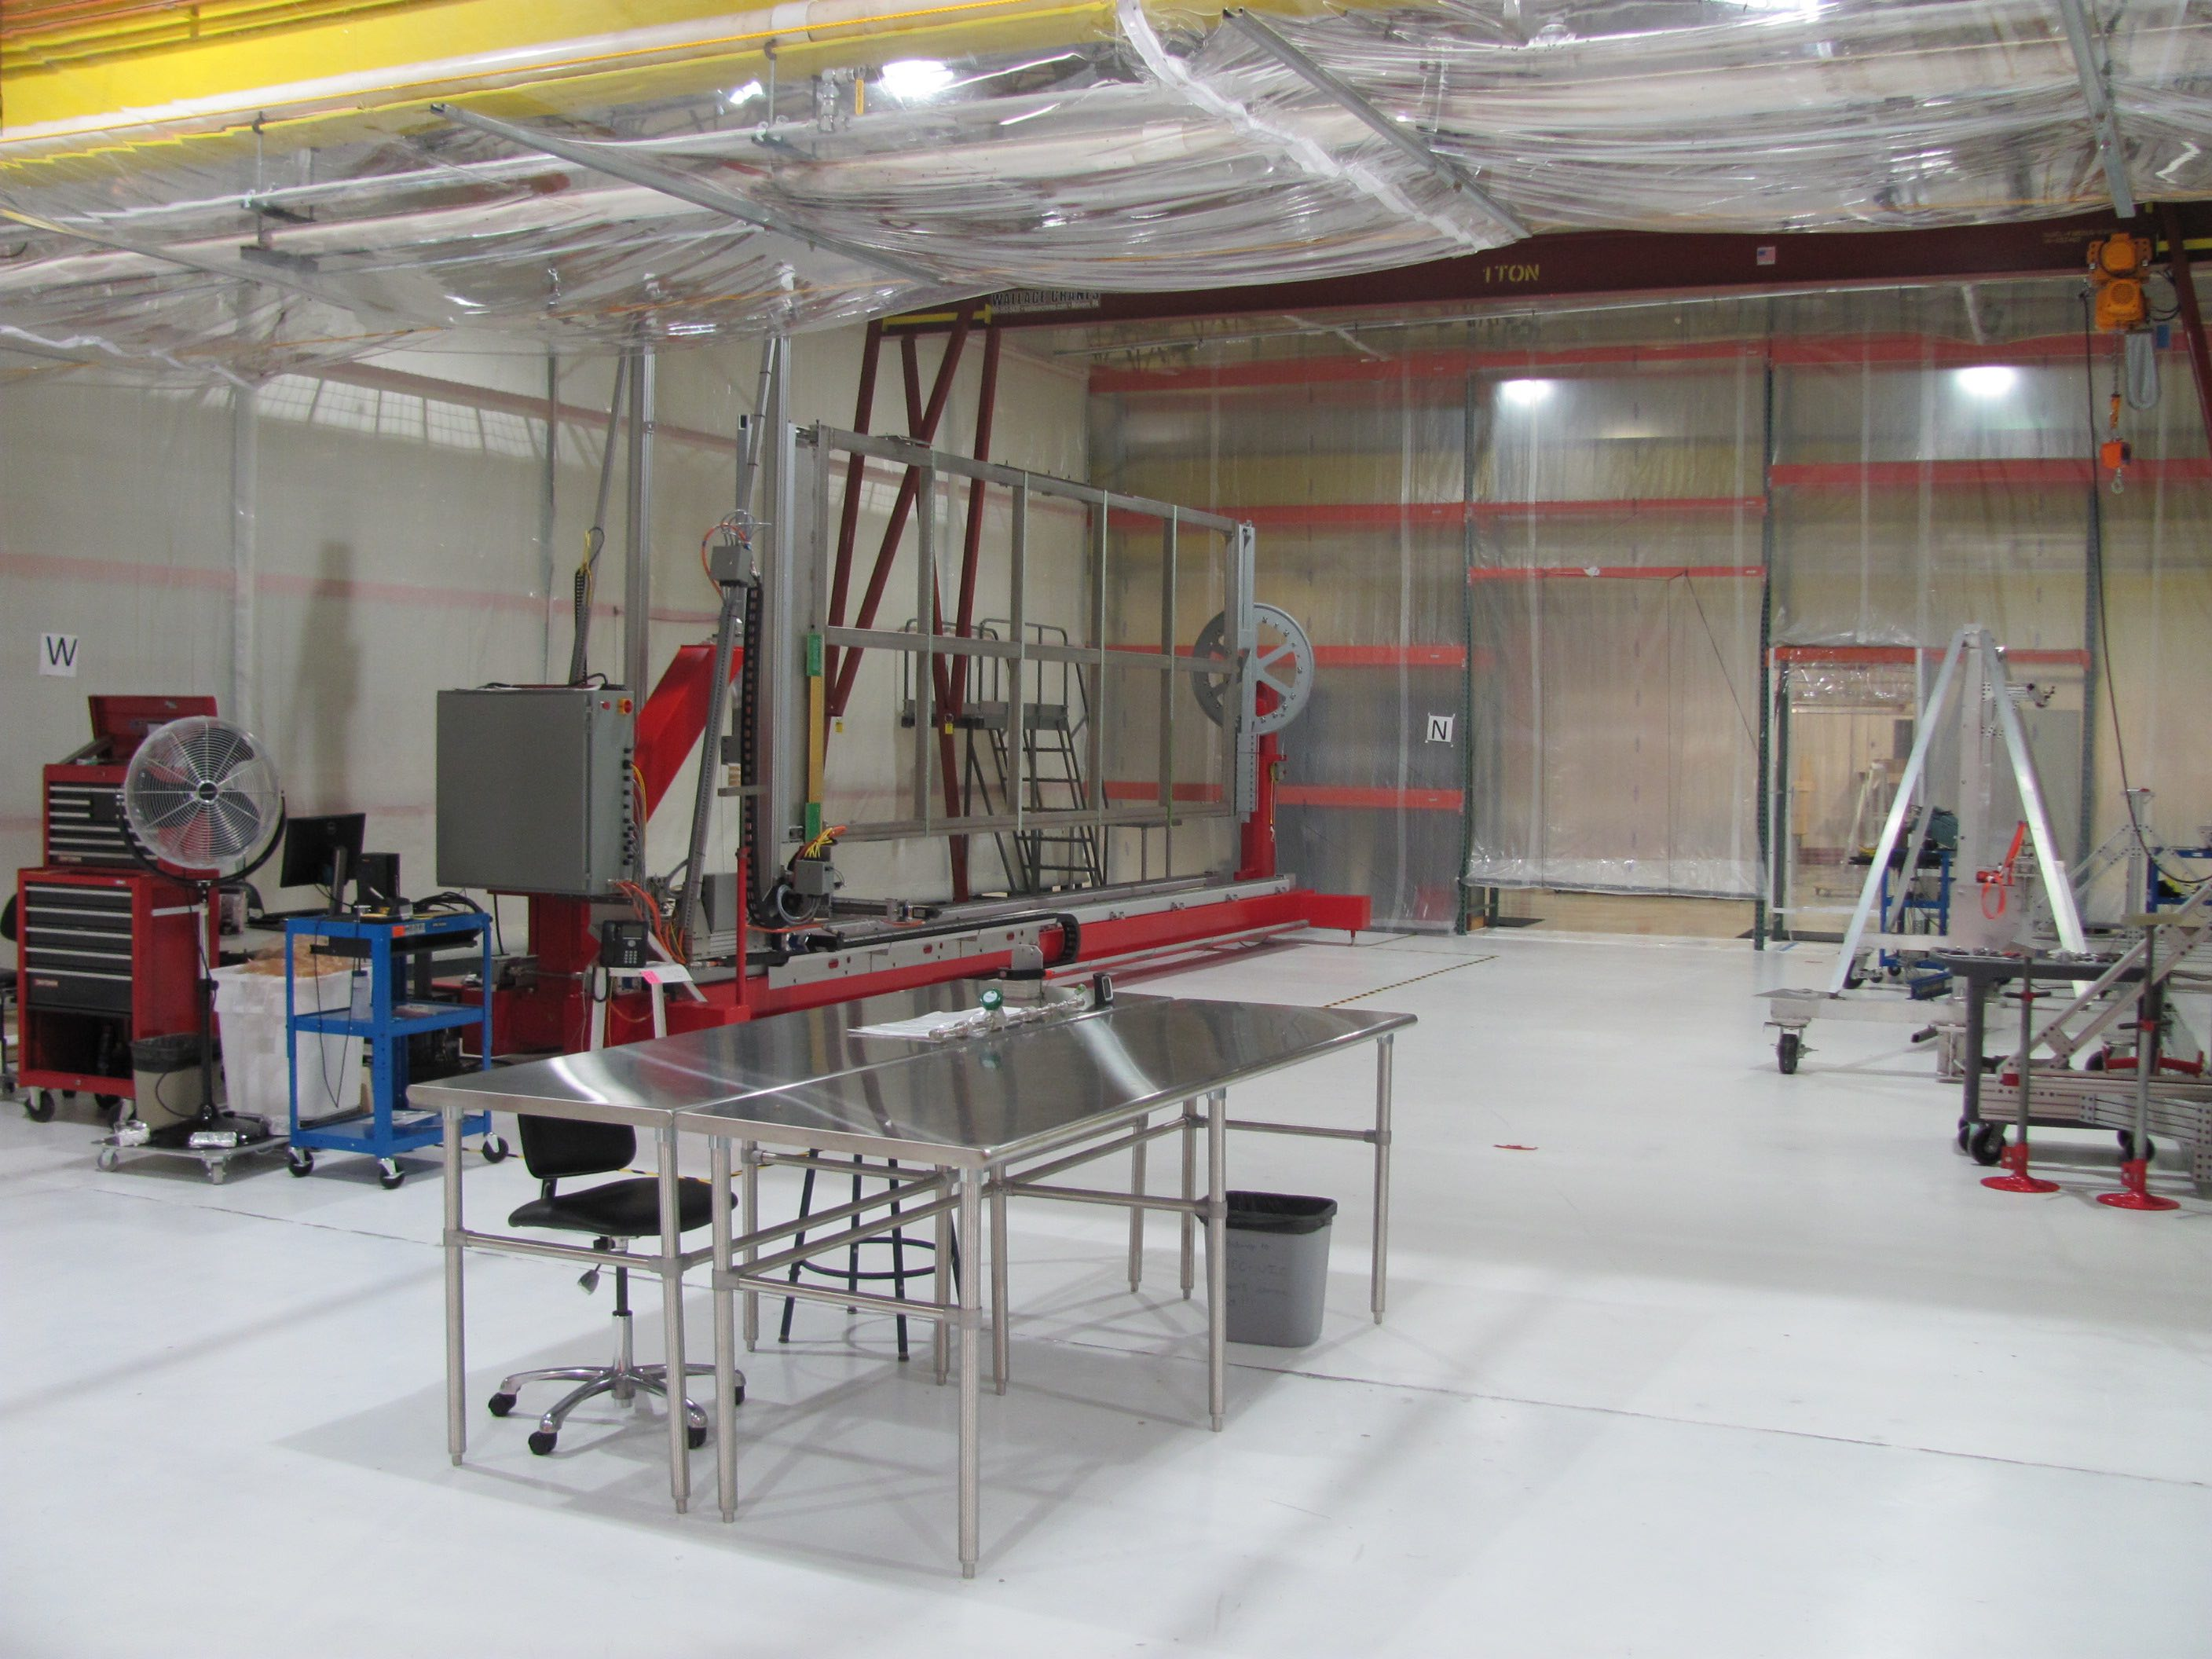
\includegraphics[height=0.225\textheight]{sp-apa-factory-psl.jpg} 
\end{dunefigure}

In the USA, there will be six total production lines at three sites: two at the University of Chicago, two at Yale University, and two at the University of Wisconsin's PSL, including the existing winder where the construction for \dword{pdsp} was carried out. 

The \dword{apa} production site at the University of Chicago will be housed in the Accelerator Building on campus in Hyde Park.  The building has hosted the assembly of large apparatus for numerous experiments over the course of its history and features an extensive high bay with an overhead crane, an indoor truck bay, clean laboratory spaces, a professional machine shop, and proximity to faculty and staff offices.  Winding will be done inside a clean room installed on the first floor-level mezzanine, where there is \SI{234}{m^2} of floor space above the machine shop.  A \SI{2}{ton} capacity bridge crane will be installed inside this clean room to move \dword{apa}s to and from the two winders and process carts that will be located here.  \dword{apa}s will enter and exit the mezzanine by way of a loading deck external to the clean room.  Preparation of \dword{apa} frames, including mesh installation, will be done inside a second clean room on the basement level floor of the high bay.  Ample space, roughly \SI{170}{m^2}, between this clean room and the truck bay allows for simultaneous receiving of bare frames or other larger items, hoisting of \dword{apa}s to and from the mezzanine, and packaging of completed \dword{apa}s for outbound shipment.  When needed, additional off-site storage will be available for holding excess inventory and completed \dword{apa}s before they are transported to South Dakota.

Yale's Wright Laboratory will host another of the USA-based \dword{apa} production sites in a recently renewed area named ``The Vault'' where the nuclear accelerator operated previously.  The Vault is approximately \SI{720}{m^2} of total floor space and it satisfies all the safety and space requirements to be an \dword{apa} production site. 
Indeed, the area, which is planned to be completely transformed into a clean room, can easily host two winders and four processing carts and has sufficient space for crating the \dword{apa}s for shipments and receiving and stocking all the material such as bare frames, electronics boards, mesh panels, and so on. There is a large high bay door at one end with direct road access which allows trucks to back inside the room where a \SI{10}{ton} crane operates all along the length.  Moreover, Wright laboratory has good support infrastructure such as clean rooms and modern mechanical and prototyping workshops that are directly connected to the Vault. Faculty, researchers and postdoc offices are located in the same building right upstairs from the Vault.

The Physical Sciences Laboratory (PSL) Rowe Technology Center has up to \SI{1850}{m^2} (\SI{20000}{ft^2}) total space available for continued \dword{dune} activities.  A clean work area that houses the existing winding machine used for \dword{pdsp} is already in place and will be used for \dword{dune} \dword{apa} construction. A second \dword{apa} production line using the updated winder design will assembled in 2020, and the existing winder will be upgraded.  PSL will host other major activities as well, including the assembly of bare \dword{apa} frames for wiring in the USA, production of \dword{cr} boards, and fabrication of \dword{apa} pair linkage and installation hardware.

Development work relevant for local planning at each site is rapidly advancing.  Figure~\ref{fig:factories} shows current conceptual layouts for the future production setups at Daresbury, Chicago, and Yale and a photograph of the existing \dword{apa} production facility at PSL-Wisconsin.  Production Site Design Reviews of the Chicago and Yale facilities are planned for early in 2020. % and Production Site Readiness Reviews are anticipated for December 2020, followed by the start of \dword{apa} production in the USA in January 2021.  
 

%%%%%%%%%%%%%%%%%%%%%%%%%%%%%%%%%%%%%%%%%%%%%%%%%%%%%%%%%%%%%%%%%%%%%%%%%%%
\subsection{Material Supply}  
\label{sec:fdsp-apa-prod-supply}
%%%%%%%%%%%%%%%%%%%%%%%%%%%%%%%%%%%%%%%%%%%%%%%%%%%%%%%%%%%%%%%%%%%%%%%%%%%

Ensuring the reliable supply of raw materials and parts to each \dword{apa} production site is critical to keeping \dword{apa} production on schedule through the years of construction. Here the consortium institutions are pivotal in taking responsibility for delivery of \dword{apa} sub-elements. Supplier institutions will be responsible for sourcing, inspecting, cleaning, testing, quality assurance, and delivery of hardware to each production site.  In particular, the critical activities to supply production sites with the minimum needed \dword{apa} components for assembly include:

\begin{itemize}

\item {\bf Frame construction:} There will be separate sources of frames in the USA and the UK. The institutions responsible will rely on many lessons learned from \dword{pdsp}. The effort requires specialized resources and skills, including a large assembly area, certified welding capability, large scale metrology tools and experience, and large-scale tooling and crane support. We are considering two approaches for sourcing: one is to outsource to an industrial supplier; the other is to procure all the major machined and welded components and then assemble and survey in-house. Material suppliers have been identified and used with good results on \dword{pdsp}.

\item {\bf Grounding mesh supply:} The modular grounding mesh frame design allows the mesh screens to be produced outside of the \dword{apa} production sites and supplied for \dword{apa} construction.  Suitable vendors to supply the needed units (20 mesh frames per \dword{apa}) will be identified in both the USA and UK.   %Elsewhere in this proposal, we describe the current mesh installation procedure. However, our \dword{pdsp} experience leads us to believe that moving to smaller self-supporting \textit{window screen} panels may save assembly time and improve overall \dword{apa} quality. We have an excellent source of mesh that was used on \dword{pdsp}.

\item {\bf Wire wrapping board assembly:} Multiple consortium institutions will take on the responsibility of supplying the tens of thousands of wire-wrapping boards required for each \dword{sp} \dword{detmodule}. The side and foot boards with electrical traces are procured from suppliers and a separately bonded tooth strip is installed to provide wire placement support. %The \num{150} \dwords{apa} require \num{276} boards per \dword{apa}, or \num{41400} boards total. 
The institutions responsible for boards will work with several vendors to reduce risk and ensure quality. 

%\item Capacitive-resistive boards: These boards are unique given their thickness, 
%\dword{hv} components, and leakage current requirements. A reliable source of bare boards was found for \dword{pdsp}. Assembly and testing was performed at PSL. We will conduct a more exhaustive search for vendors willing to take on assembly and testing for the \num{3000} \dword{cr} boards needed for each \dword{sp} \dword{detmodule}.

\item {\bf Wire procurement:} Wire is a significant element in the assembly of an \dword{apa}. Approximately \SI{24}{km} of wire is wound onto each unit. During \dword{pdsp}, %we have worked with 
an excellent supplier %that 
has worked with us to provide high quality wire wound onto spools that we provide. These spools are then used directly on the winder head with no additional handling or re-spooling required. Wire samples from each spool are strength tested before use.

\item {\bf Comb procurement:} Each institution will either work with our existing comb supplier or find other suppliers who can meet our requirements. The \dword{pdsp} supplier has been very reliable.

%\item Winders and tooling: We propose that PSL and Daresbury work together to supply tooling and winding machines for additional production lines at new locations and for additional lines in-house. This natural collaboration has been in place for nearly two years for \dword{pdsp}.

\end{itemize}


%%%%%%%%%%%%%%%%%%%%%%%%%%%%%%%%%%%%%%%%%%%%%%%%%%%%%%%%%%%%%%%%%%%%%%%%%%%
\subsection{Quality Control in APA Production}
\label{sec:fdsp-apa-prod-qc}
%%%%%%%%%%%%%%%%%%%%%%%%%%%%%%%%%%%%%%%%%%%%%%%%%%%%%%%%%%%%%%%%%%%%%%%%%%%

%\fixme{Justin, Mitch, Roxanne: review text}

%A key part of \dword{qa} for the \dword{apa} design and manufacturing procedures is the experience with \dword{pdsp}, including upcoming operations and data analysis results from the detector.  We have already learned much about design, component testing, and fabrication procedures that will help in formulating the detailed design and plans for the DUNE \dword{apa} construction project over the next year.  The set of final design drawings and detailed procedures documentation generated over the next year leading to the \dword{tdr} represent an important element of the \dword{qa} plan for fabricating the \dwords{apa}.  

%Summaries of all \dword{qa} testing performed on elements used in the final design of the \dwords{apa} will also be prepared for the \dword{tdr}.  Much data already exists, and again, \dword{pdsp} will provide valuable additional information on the robustness of the detector components and construction.  

\Dword{qc} testing is a critical element of \dword{apa} production.  All \dword{qc} procedures are being developed by the consortium and will be implemented identically at all production sites in order to ensure a uniform quality product as well as uniform available data from all locations.  Important \dword{qc} checks are performed both at the level of components, before they can be used on an \dword{apa}, as well as on the completed \dword{apa}s, to ensure quality of the final product before leaving the production sites.  In addition, a 10\% sample of the completed \dword{apa}s produced at each of the production sites each year will be cold cycled in a cryogenic test facility available at PSL.

\subsubsection{APA Frame Acceptance Tests} 

Each \dword{apa} support frame must meet geometrical tolerances in order to produce a final \dword{apa} that meets requirements for physics. In particular, the wire plane-to-plane spacing must be within the specified tolerance of $\pm$\SI{0.5}{mm} (see Sec.~\ref{sec:fdsp-apa-design-overview}).  Flatness of the support frame, therefore, is a key feature and is defined as the minimum distance between two parallel planes that contain all the points on the surface of the \dword{apa}.  Although there are any number of ways in which the frame could be distorted out of plane, the most likely ones can be approximated by three modes: 1)~a curve in the long side tubes causing the frame to bow out of plane, 2)~a twist in the frame from one end to the other, and 3)~a fold down the center-line (if the ends of the ribs are not adequately square).

As detailed in Section~\ref{sec:fdsp-apa-frames}, \dword{apa} frames are constructed of 13 separate rectangular hollow steel sections.  Before machining, a selection procedure is followed to choose the sections of the steel most suited to achieving the geometrical tolerances.  After assembly, a laser survey will be performed on the bare frames before they can be delivered to an \dword{apa} production site. Three sets of data are compiled into a map that shows the amount of bow, twist, and fold in the frame. A visual file is also created for each \dword{apa} from measured data. 

A study was performed to determine the tolerances on the three distortions characterized above and is documented in~\cite{bib:docdb1300}.  It was determined that a \SI{0.5}{mm} change in the final wire plan spacing could result from:
\begin{enumerate}
\item An \SI{11}{mm} out-of-flatness caused by curved long side tubes.
\item A \SI{6}{mm} out-of-flatness due to a twist in the frame.  This is assumed to be evenly distributed between each of the 5 cells of the \dword{apa} with $\sim$\SI{1.2}{mm} out-of-flatness per cell.
\item A \SI{1.2}{mm} out-of-flatness due to a fold down the middle of the \dword{apa}.
\end{enumerate}

The bow, twist, and fold extracted from the survey data will be compared against these allowable amounts before the support frame is used to build an \dword{apa}.  Later, during \dword{apa} wiring at the production sites, a final frame survey will be completed after all electrical components have been installed, and the as-built plane-to-plane separations will be measured to verify that the distance between adjacent wire planes meets the tolerances.  

Another check performed at the \dword{apa} production site before the frame is transferred to a winder will confirm sufficient electrical contact between the mesh sub-panels and the \dword{apa} support frame.  A resistance measurement is taken immediately after mesh panel installation for all \num{20} panels before wiring begins.


%The following \dword{qc} data are to be collected for each \dword{apa} during production:  

%\begin{itemize}

%\item Frame flatness: A laser survey measures the flatness of the assembled bare frame. Three sets of data are compiled into a map that shows the amount of bow, twist, and fold in the frame. Each of these parameters is compared to an allowable amount that does not cause wire plane-to-plane spacing to be out of tolerance ($\pm$\SI{0.5}{mm}).  A visual file is created for each \dword{apa} from measured data. A final frame survey is completed after all electrical components have been installed, and the as-built plane-to-plane separations are measured to verify the distance between adjacent wire planes.

%\item Mesh to frame connection: To confirm sufficient electrical contact between the mesh sub-panels and the \dword{apa} support frame.  A resistance measurement is taken immediately after mesh panel installation for all \num{20} panels before winding begins.

%\item Wire tension: The tension of each wire is measured after each new plane of wires is installed on an \dword{apa}. The optimal target tension has been updated to \SI{6}{N} based on \dword{pdsp} experience.  \Dword{pdsp} data, where the tensions have substantial variation, will provide important input for quantifying the effects of varying tensions and finalizing the allowed range of values.  
%Wire tensions must be in the range 3.5--\SI{7.5}{N} for wires longer than \SI{750}{mm} and in the range 2.0--\SI{7.5}{N} for wires shorter than \SI{750}{mm}.
%\item Cleanliness: \dwords{apa} are produced inside a class 100,000 clean area.  Particle counts are completed daily to verify cleanliness of the assembly area.  If counts fall outside expected limits, measures are taken to re-clean the affected area and check with another particle count.
%\end{itemize}


\subsubsection{Material Supply Inspections}

%\fixme{add about the plan to do component testing via work packages.  is it the same in the UK? talk about the importance of not starving the factories for parts and that the parts must show up confirmed for use on an APA.}

All components require inspection and \dword{qc} checks before use on an \dword{apa}.  Most of these tests will be performed at locations other than the \dword{apa} production sites by institutions within the consortium before the hardware is shipped for use in \dword{apa} construction. This distributed model for component production and \dword{qc} is key to enabling the efficient assembly of \dword{apa}s at the production sites.   The critical path components are the support frames (1 per \dword{apa}), grounding mesh panels (20 per \dword{apa}), and wire carrier boards (204 per \dword{apa}). Section~\ref{sec:fdsp-apa-org} provides details about which consortium institutions in the US and UK will be responsible for each of these work packages.  

\begin{comment}
\begin{itemize}
%\item Frame components: If \dword{apa} steel frames are produced in-house, then upon receipt of the rectangular hollow section steel for the frames, a selection procedure is followed to choose the sections of the steel most suited to achieving the geometrical tolerances.

\item Wire testing: The CuBe wire is provided on spools from the supplier. Samples from each spool are strength tested before use on an \dword{apa}.

\item Circuit boards: All circuit boards installed on an \dword{apa} are inspected for dimensional accuracy before being routed through various epoxy and cleaning processes as they are prepped for assembly. Inspection results are documented, and if anomalies are found, an electronic non-conformance report is written.  %Materials that can be re-worked to become conforming are set aside from inventory and re-worked.  If the material cannot be made usable, the material is kept in a non-conforming area sequestered from usable inventory.   

\item \dword{cr} and $G$-plane bias board testing: Acceptance tests of these boards include leakage current measurements ($<$\SI{0.5}{nA}) and continuity tests on each channel.  The tests are performed at room temperature. \dword{pdsp} was used to perform design validation on more than \num{100} boards that were cycled and tested at \lntwo temperature. No failures were seen during these tests. 
\end{itemize}
\end{comment}

\subsubsection{Wire Tension Measurements and Channel Continuity and Isolation Checks}
\label{sec:fdsp-apa-prod-qa-tension}

The tension of every wire will be measured during production to ensure wires have a low probability of breaking or moving excessively in the detector.  Every channel on the completed \dword{apa}s will also be tested for continuity across the \dword{apa} and isolation from other channels.  The plan is to perform all tests at once, using the methods described in this section.  As will be described in Section~\ref{sec:fdsp-apa-prod-coldtest}, it is also planned that 10$\%$ of the \dword{apa}s will be shipped to PSL for a cold test, where the full \dword{apa} will be brought to liquid nitrogen temperature. Following the cold test, the wire tensions and continuity will be remeasured.  Finally, for this 10$\%$ sample of \dword{apa}s, a measurement of the wire plane spacing will be performed using a Faro arm that can precisely record the position of each wire plane in space. This checks that the quality control on the flatness of the support frames remains sufficient.  

Wire tensions will be measured after each new plane of wires is installed on an \dword{apa}. The optimal target tension has been set at \SI{6}{N} based on \dword{pdsp} experience.  \Dword{pdsp} data, where the tensions did have substantial variation, is also being used to study the effects of varying tensions and finalize the allowed range of values.  
%Wire tensions must be in the range 3.5--\SI{7.5}{N} for wires longer than \SI{750}{mm} and in the range 2.0--\SI{7.5}{N} for wires shorter than \SI{750}{mm}.
%\item Cleanliness: \dwords{apa} are produced inside a class 100,000 clean area.  Particle counts are completed daily to verify cleanliness of the assembly area.  If counts fall outside expected limits, measures are taken to re-clean the affected area and check with another particle count.

% An area for potential improvement in the construction process that could make \dword{apa} fabrication more efficient and reliable is the technique used to measure wire tensions.  Individual wire tension can be determined by measuring the resonant vibration frequency of a wire that has been mechanically disturbed.  The current technique involves manually plucking the wires and using a laser photodiode tool mounted on the winder to measure tension one wire at a time.  This takes many hours for each wire plane. A task force within the consortium was recently initiated to study the problem and consider possible new approaches to measuring tension. In particular, methods to electronically disturb and measure groups of \num{20} or more wires at one time have recently been explored, so the task force is studying the feasibility of applying this during \dword{apa} construction. The recent developments, where an electronics board has been designed to supply the voltages to multiple wires while reading out the resonance frequency of vibration of the measured wires, have shown promising results. Scanning the wire tension of a full wire plane should take only a few minutes. Further tests and studies are required to validate the electrical methods, and a final prototype should be available soon. With such a less labor intensive and faster method, it also becomes possible to measure more of the wire tensions later in the construction of the detector, for example during integration and installation at \dword{surf}. 

The technique %customarily used to measure the wire tension in an \dword{apa} is based on a laser and a photodiode~\cite{Acciarri:2016ugk}. In particular, this is the technique that 
used to measure tensions for the \dword{apa}s of \dword{pdsp} was based on a laser and a photodiode system~\cite{Acciarri:2016ugk}. In this method, the laser shines on an individual wire and its reflection is captured by the photodiode. An oscillation is produced in the measured voltage when a vibration is induced on the wire, such as by manually plucking it. This oscillation is dominated by the fundamental mode of the wire, which is set by the wire's tension. Since the length and density of the wire are known, the measured fundamental frequency can be converted into a tension value. The method works very well, but due to the necessity of aligning the laser and exciting and measuring wires individually, this technique can take tens of seconds per wire. Given the large number of wires per \dword{detmodule}, development of a faster technique represents a major opportunity for the full \dword{dune} construction.

A technique that can reduce the overall time required to measure the tension of every wire is currently being developed~\cite{Garcia-Gamez:2018frz}. In this method, DC and AC voltages are applied on the neighbouring wires of a wire under test. A sine wave of the same frequency as that of the applied AC voltage is measured from the tested wire, since it is capacitively coupled to its neighbours. The amplitude of the sine wave exhibits a resonant behavior when the frequency of the AC voltage corresponds to the fundamental frequency of the wire. Thus, a frequency sweep of the AC voltage can be performed to determine at which frequency there is a resonance, from which the wire tension can be obtained. As electrical signals can be injected and measured in several wires simultaneously, this technique has the potential of measuring the tension of many wires at once.

A wire tension measurement device based on the electrical method is being developed within the context of the \dword{dune} \dword{apa}s. While the underlying principle of the electrical method has been demonstrated, its technical implementation requires consideration. The wire pitch of the \dword{apa}s requires summed input voltages on the order of \SI{500}{V} to reasonably discern resonances against noise. The head boards, cf.\ Section~\ref{sec:fdsp-apa-headboards}, have been designed to withstand temporarily such large differential voltages across neighbouring channels. Additionally, the components of the \dword{cr} boards or of the cold electronics would interfere with the method and need to be absent.
%Dedicated contact pads on the head boards have been added, in proximity to those for the \dword{cr} boards, for the measurement device to connect electrically to the wires.

The exact specifications of the measurement system are being finalized. It is planned to connect to one of the twenty head board stacks at a time. Within a given stack, the device is projected to inject and read out signals by groups of sixteen wires simultaneously. The device could be used to measure the tension of any wire layer at any stage of the production process, in particular after the winding of a wire layer or after all the wires are wound. The designs of the winder machine and of the \dword{apa} protection panels have clearance provisions for the usage of such a measurement device.

The measurement system design is a combination of a commercial \dword{fpga} board and a custom printed circuit board for analog signal processing. An \dword{fpga} board is used as it can produce a square wave at any frequency that is expected to be encountered while measuring a wire's fundamental frequency, i.e.,\ below \SI{5}{kHz}. In addition, the \dword{fpga} board can be used for digital signal processing of the readout signal. The analog circuitry would act as a bridge between the \dword{fpga} and the \dword{apa} wires. It is needed to filter the square wave into a sine wave, to amplify that sine wave before sending it to the wires and to digitize the readout signal before sending it to the \dword{fpga}. The analog board is also needed to provide electrical connections to the head boards. With such a design, it is expected that the concurrent tension measurement of eight wires would take on the order of ten seconds.

A prototype of the measurement device has been built. The main difference between the prototype and the planned design is that the former is restricted to three wires instead of sixteen: a single readout wire and two stimulus wires. The prototype has been employed on a test bench in which wires with the same physical properties as those that will be used in the \dword{apa}s have been wound. The wires were wound according to these wire parameters, which are similar to those of the \dword{apa}s: \SI{6}{N} tension, \SI{6}{m} length, \SI{4.7}{mm} pitch. The applied voltages were \SI{400}{V} DC and \SI{26}{V} for the AC peak amplitude. The results obtained are shown in Figure~\ref{fig:electrical-tension}. The expected resonant frequency is \SI{16.1}{Hz}. The observed resonant frequency is obtained from the raw data by offline data analysis using numerical algorithms that can be implemented directly in the \dword{fpga}. The value obtained is \SI{16.0}{Hz}, corresponding to a tension value of \SI{5.9}{N}, which is within a few percent of the physical value.

\begin{dunefigure}[Observed resonant frequency in electrical wire tension method]{fig:electrical-tension}
{Amplitude of the readout signal as a function of the stimulus frequency, as used in the electrical wire-tension method. The vertical line is located at the observed resonant frequency. The raw digitized signal values corresponding to the first data point of the main plot are shown in the inset plot.}
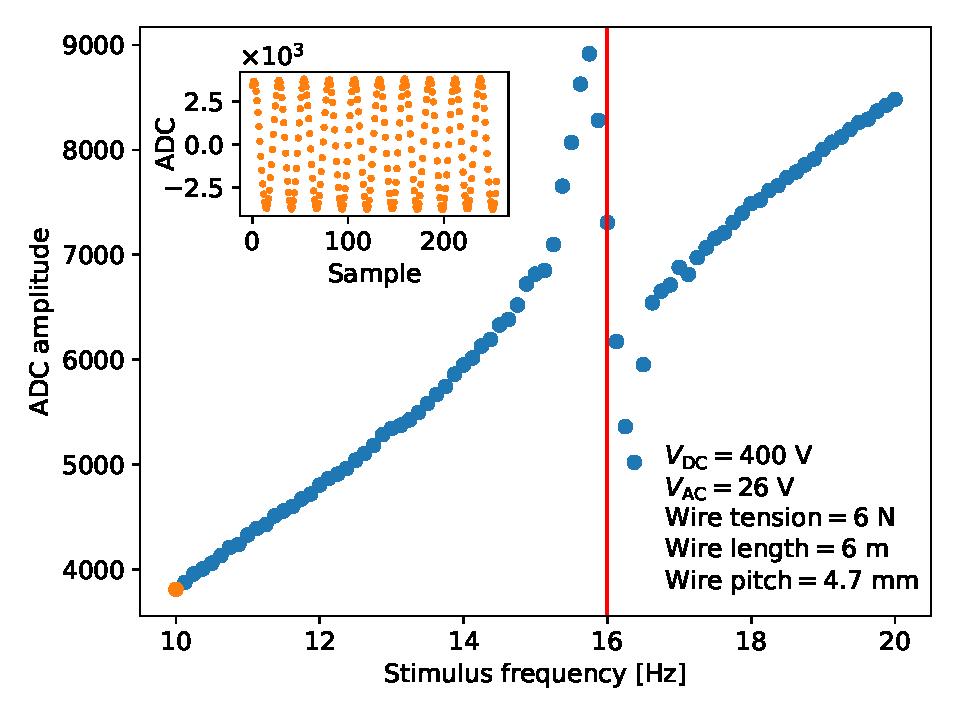
\includegraphics[height=0.33\textheight]{sp-apa-electrical-tension.pdf}
\end{dunefigure}

In this test bench setup, no wire support combs, cf.\ Section~\ref{sec:combs}, are present. Their presence shortens the wire length that needs to be considered in this method, resulting in several higher resonant frequencies per wire. A similar effect happens for the wire channels that wrap around the \dword{apa} frame. Although they are a succession of wire segments electrically connected, the segments are mechanically independent and can have different tension values. Several resonant frequencies can be present per readout channel, possibly corresponding to different tension values.

In addition to measuring tension values, the measurement device is envisioned to be able to test wires for electrical isolation and electrical continuity, given the flexibility of the \dword{fpga} and provisions put in place in the design of the analog circuitry. Injecting a signal in a readout channel and detecting it in a different channel would indicate that these channels are not electrically isolated, for example, due to a solder bridge. The electrical continuity could be tested by sending a pulse down a channel and measuring the time it takes to travel through the wire and back to the measurement device.  If the measured time is shorter than expected, this could indicate cold solder joints, for example.

A final review of the electrical tension measuring system design will take place in spring 2020. Once completed, mobile \dword{apa} test stands will be built for each of the \dword{apa} production sites, the \dword{sdwf}, and \dword{surf}.  The introduction of the electrical testing methods for \dword{apa}s presents a fantastic opportunity for more efficient \dword{apa} fabrication and more flexible testing during the integration and installation phases.    


\subsubsection{Cold Testing of APAs}
\label{sec:fdsp-apa-prod-coldtest}

The six \dword{apa}s produced for \dword{pdsp} have demonstrated clearly that the \dword{apa} design, materials, and fabrication methods are sufficiently robust to operate at liquid argon temperature.  No damage or change in performance due to cold have been identified during \dword{pdsp} running.  Nevertheless, over a five year construction effort, it is prudent to cold cycle a sample of the \dword{apa}s produced to ensure steady fabrication quality.  A cold testing facility sized for \dword{dune} \dword{apa}s exists at PSL and can be used for such tests. Throughout the construction project, it is anticipated that 10\% of the produced \dword{apa}s will be shipped to PSL for cold cycling.  This amounts to about 1 APA per year per production site during the project.  It is planned that all APAs will still be cold tested during integration at SURF and before installation in the DUNE cryostats.      


\subsubsection{Documentation} 
\label{sec:fdsp-apa-prod-doc}

Each \dword{apa} is delivered with a traveler document in which specific assembly information is gathered, initially by hand on a paper copy, then entered into an electronic version for longer term storage.  The traveler database contains a detailed log of the production of each \dword{apa}, including where and when the \dword{apa} was built and the origin of all parts used in its construction. 

Assembly issues that arise during the construction of an \dword{apa} are gathered in an issue log for each \dword{apa}, and separate short reports provide details of what caused the occurrence, how the issue was immediately resolved, and what measures should be taken in the future to ensure the specific issue has a reduced risk of occurring.  


%%%%%%%%%%%%%%%%%%%%%%%%%%%%%%%%%%%%%%%%%%%%%%%%%%%%%%%%%%%%%%%%%%%%%%%%%%%
%%%%%%%%%%%%%%%%%%%%%%%%%%%%%%%%%%%%%%%%%%%%%%%%%%%%%%%%%%%%%%%%%%%%%%%%%%%